
\chapter{Problem-solving and diagnostic strategies}

The ability to solve complex problems is the most valuable technical skill an instrumentation professional can cultivate.  A great many tasks associated with instrumentation work may be broken down into simple step-by-step instructions that any marginally qualified person may perform, but effective problem-solving is different.  Problem-solving requires creativity, attention to detail, and the ability to approach a problem from multiple mental perspectives.

``Problem-solving'' often refers to the solution of abstract problems, such as ``word'' problems in a mathematics class.  However, in the field of industrial instrumentation it most often finds application in the form of ``troubleshooting:'' the diagnosis and correction of problems in instrumented systems.  Troubleshooting is really just a form of problem-solving, applied to real physical systems rather than abstract scenarios.  As such, many of the techniques developed to solve abstract problems work well in diagnosing real system problems.  As we will see in this chapter, problem-solving in general and troubleshooting in particular are closely related to \textit{scientific method}, where hypotheses are proposed, tested, and modified in the quest to discern cause and effect.

Like all skills, problem-solving may be improved with practice and persistence.  The goal of this chapter is to outline several problem-solving tools and techniques.








\filbreak
\section{Learn principles, not procedures}

\begin{quote}

``As to methods there may be a million and then some, but principles are few.  The man who grasps principles can successfully select his own methods.  The man who tries methods, ignoring principles, is sure to have trouble.'' -- \textbf{Ralph Waldo Emerson}  \index{Emerson, Ralph Waldo}

\end{quote}

Effective problem-solvers always reason from fundamental principles, rather than follow memorized procedures.  Following this logic, the wise strategy for any student learning how to solve any type of problem is to internalize as many general principles as possible, and to connect common threads of principle to different applications and scenarios.

A good way for any student to self-check that their focus is indeed on principles rather than procedures is to continually ask themselves if they are able to explain \textit{why} what they have learned is true.  It is one thing to be able to explain what you have learned, but it is quite another to explain \textit{why} your new knowledge is valid.  ``Why'' may be the most important question you ever ask, and you need to ask it often.

% ADD: illustrative examples?










\filbreak
\section{Active reading}

\index{Active reading}  \index{Reading, active}

Learning from reading printed text is a kind of problem-solving activity it is own right.  The problem is how to acquire new information from the pages of a book, and the solution requires active engagement of your mind as you read.  This is often more difficult that it may seem at first, especially when the subject matter is complex and/or the source text is poorly written.  Given the fact that much more technical information is available in text form than in any other format, and also the fact that continuous learning is absolutely essential in the field of instrumentation, active reading is an indispensable tool for student success as well as for continued professional growth in the field of instrumentation.






\filbreak
\subsection{Don't limit yourself to one text!}

A very common mistake made by struggling students is to limit themselves to the reading assigned by their instructor(s), when better books might be available.  If homework assignments are given from a particular assigned text, it is understandable why a student might think this is the \textit{only} appropriate text to use.  However, textbook selection is an imperfect process, often influenced by factors other than optimal learning (e.g. instructor bias, publisher influence, etc.).  Sadly, textbooks are sometimes chosen not on their merits as a learning resource but rather by whether or not the textbook comes complete with pre-made exercises and examinations to be used in class (thus relieving the instructors of much work creating these on their own).  As a student you must take responsibility for your own learning and seek the best books available for learning, even if this means only using the assigned text as a source of homework problems!

\vskip 10pt

Thanks to the internet, searching for high-quality books is very easy.  Not only may you peruse titles and reviews, but many booksellers also allow limited access to these texts online so you can see firsthand how the books are written and decide whether or not each book would suit your needs.

If you are a student and you approach your instructor asking about other texts to read on the subject, you may find your instructor doesn't like the assigned text any better than you, and has alternatives ready to suggest.  This is often the case in courses where the text has been selected by committee.

\vskip 10pt

If you examine the personal library of any highly competent technician or engineer, you will likely find multiple books covering the same topics.  Building your own collection of useful texts for learning is a sound strategy.  Not only will you find yourself referencing these books throughout your career, but you will find their multiple explanations of common concepts an easier way to learn than by limiting yourself to just one point of view.









\filbreak
\subsection{Marking versus outlining a text}

A practical and common method to increase engagement while reading is to ``mark'' the paper pages of a book with notations, the idea being to note points of interest and thereby stimulate thinking as you read.  For a brief primer on this subject I recommend Mortimer Adler's essay \textit{How to Mark a Book}. 

\vskip 10pt

We will begin our exploration of active reading with an example taken from page 101 of the classic text \textit{The Measurement of High Temperatures} written by George Burgess and Henry Louis Le Ch\^{a}telier in 1912.  One reason for choosing such an old text is that the style of writing adds another challenge to the task of reading.  For those already familiar with the subject of temperature measurement, the archaic writing style will help give you the perspective of a new student, encountering something unfamiliar for the first time:  \index{Burgess, George}  \index{Le Ch\^{a}telier, Henry Louis}

$$\includegraphics[height=5in]{activereading_1.eps}$$

This is the original text as it appears on page 101 of the book.  Next, we will explore different ways of ``marking'' the text, as if we were a new reader to this subject.

\filbreak

The most rudimentary method of marking a book consists of underlining and/or highlighting with a felt-tipped pen:

$$\includegraphics[height=5in]{activereading_2.eps}$$

Here you see how the reader has highlighted the paragraph introductory words in yellow ink, underlined names and dates with green lines, and underlined concepts with red lines.  While such exercises may have helped the reader remain awake as well as generate cues for later cramming, it is doubtful they assisted the reader in understanding the concepts.  A large degree of blame for this rather shallow and unproductive practice may be laid on instructional curricula emphasizing memorization and execution of procedures over conceptual understanding.  Simply put, \textit{this is what you get when students expect to be quizzed on isolated bits of data:} you get poor study habits such as this.  Unfortunately, not only will this approach fail to yield deep understanding of the concepts, but it also reduces the act of reading to drudgery.  When such practices are so common, it's no wonder a great many students loathe academic reading.

\filbreak

The choice of highlighting versus underlining, or of one color over another, is relatively unimportant.  Any process of ``marking'' a book merely by drawing attention to certain words within it suffers the same weakness: all you are doing is emphasizing specific words and phrases, not incorporating your own thoughts into the text.  In order to be \textit{actively engaged} in your reading, you must expose your own thoughts and reflections on what you read, not just emphasize specific statements made by the author.  As Adler points out:

\begin{quote}

``Understanding is a two-way operation; learning doesn't consist in being an empty receptacle.  The learner has to question himself and question the teacher.  He even has to argue with the teacher, once he understands what the teacher is saying.  And marking a book is literally an expression of differences, or agreements of opinion, with the author.''

\end{quote}

The thrust of Adler's essay is that the reader gains the greatest understanding of a text by expressing their own thoughts about what they are reading: articulating questions, drawing conclusions, linking ideas, and otherwise being an active participant in the reading process rather than a passive observer.

\vskip 10pt

\filbreak

With this in mind, let's re-approach the text.  Instead of simply emphasizing words and phrases, we will now show how a reader may articulate some of their own thoughts on the same page:

$$\includegraphics[height=5in]{activereading_4.eps}$$

Here you can see the focus has completely shifted away from facts and figures, and toward concepts.  Note the questions raised by the reader, either doubting their own understanding of the book or the author's assertions.  These questions need not be fully resolved at the conclusion of reading.  Indeed, these may be excellent topics to raise in class once the student returns to school and has the instructor's attention.  Questions should be taken as a positive sign for active reading and not as an indication of trouble: if you read a large body of prose and have no questions of your own, you probably weren't thinking deeply enough!

\vskip 10pt

If this manner of marking the text seems messy and cluttered, one may opt to make all the notations on a separate piece of paper, or even typed into a computer for later printing and retrieval. 

\filbreak

Even deeper engagement may be achieved if one takes the time to write an \textit{outline} of ideas in the text.  This is an exercise best done on a separate sheet of paper, or using a computer.  An example is shown here, side-by-side with the original text.  Note how an outline may include graphical sketches as well as words, and how it references the page number of the source text to make it easier to go back to the source and re-read if necessary:

$$\includegraphics[width=6in]{activereading_3.eps}$$

What you see here are notes for just one page of Burgess' and Le Ch\^{a}telier's text.  Although there is no absolute rule for how detailed one's notes should be, they should be expressed in \textit{one's own words} rather than copying the author's words, and should at minimum express \textit{at least one statement and/or question from the reader per paragraph of source text}, since each paragraph typically contains a distinct idea on the topic at hand.  A complete outline of thermoelectric pyrometers would of course cover multiple pages of the source text, and not just the one page shown.  Note how the outline includes cues for future learning -- hints that there is more to this subject than what is immediately presented on this page of the text.

\vskip 10pt

Writing your own outline of a text is especially useful when the text in question is densely packed with ideas and/or difficult to understand, because the act of outlining serves as a self-check for your own comprehension.  With highlighting and underlining it is all too easy to lazily read the words and make these marks without really understanding what the text is saying.  While outlining you know quite well when you haven't understood the text because you simply won't be able to express it in your own words.  Instead of continuing to highlight in a state of blissful unawareness, you will find yourself stuck and unable to continue outlining.  This prompts you to go back and scrutinize the text, going over it more carefully than before, until you find yourself able to continue outlining again.  

Perhaps the most common objection to outlining text as you read is that the process is slow.  This raises a very important point, namely that \textit{active reading should be slow}.  Facts and figures may be skimmed, but complex ideas take time to penetrate into your mind.  Not only will outlining force you to slow down when you need to, but it will also serve as a gauge for later study when you review your own notes to see if you still agree with them.  In the course of studying some topic, you will often find that your understanding of that topic changes from your first impression.  Seeing this change for yourself allows you to better understand how you learn, and thereby gives you practical insight into the workings of your own mind when it comes time to learn something new.






%\filbreak
%\subsection{Shortening complex sentences}






%\filbreak
%\subsection{Cross-referencing}

%% ADD: reference text to diagrams
%% ADD: reference text to text






%\filbreak
%\subsection{Create your own questions}






%\filbreak
%\subsection{Identify what doesn't make sense}






%\filbreak
%\subsection{Describe problem-solving strategies modeled in the text}






%\filbreak
%\subsection{Pose experiments}

%ADD: experiments to confirm some principle
%ADD: experiments to disprove some misconception






%\filbreak
%\subsection{Describe practical outcomes}

%% ADD: what can you DO now that you could not before reading the text?









%\filbreak
%\subsection{Work through all mathematical exercises shown in the text}













\filbreak
\section{General problem-solving techniques}

A variety of problem-solving techniques have been presented for students over the years which are all helpful in tackling problems both in the classroom and in the real world.  Several of these techniques are presented here in this section.





\filbreak
\subsection{Identifying and classifying all ``known'' conditions}

An important step in solving certain types of problems, especially quantitative problems where calculations are necessary to obtain precise answers, it is often useful to list all the known quantities available to us relevant to the problem.  Similarly, taking the time to list all relevant (and possibly relevant) mathematical formulae we might apply to the solution is a helpful step.  

One way to save time applying the latter suggestion in a classroom setting is to keep a concise reference card or file filled with formulae you've been learning within that course.  This reference may be referred to as often as necessary, without having to re-write the equations for each and every problem, thus eliminating unnecessary effort.







%\filbreak
%\subsection{Identifying relevant principles}

% ADD: Common mistake: memorizing procedures instead of internalizing principles
% ADD:   "Internalizing" means not just remembering the form of a principle, but also its applicable context

% ADD: Example -- solving for thermocouple temperature using a voltmeter (V_meter = V_J1 - V_J2).
% ADD: Example -- calculating amount of fuel needed to pump quantity of water into a reservoir using an engine-driven pump







\filbreak
\subsection{Re-cast the problem in a different format}

Many people find it easier to grasp the nature of a problem -- and by extension, that problem's solution -- if they can look at an illustration of the problem.  Therefore, a helpful step in solving problems described to you in words is to translate those words into a picture to look at.  

If you are one of those people for whom drawing is a challenge, take heart in the fact that this is a skill you can build.  Practice is the key to honing this skill.  With this in mind, make it a habit to sketch some kind of illustration for every problem you are asked to solve.  If you are working in teams to solve a problem, a collaborative sketch goes a long way toward coordinating problem-solving efforts and ensuring everyone on the team has the same view of the problem.

\vskip 10pt

For some people, describing a problem verbally is helpful in solving it.  If your brain tends to work like this -- understanding concepts and situations better when they are cast into clear prose -- then you may find it helpful to first draft an explanatory paragraph of the problem in your own words.  This is also an exercise lending itself well to team-based problem solving, as the entire team can help each other describe the nature of the problem.






\filbreak
\subsection{Working backwards from a known solution}

Sometimes we may gain insight into the solution of a problem by assuming we already know the answer to a similar problem, then working ``backward'' to find the problem from that assumed solution.

An application of this problem-solving strategy is found learning how to decode binary bits that have been encoded using the Manchester standard.  With Manchester encoding, binary bits are represented by the rising and falling \textit{edges} of square-shaped waveforms rather than high and low states themselves.  For example:

$$\includegraphics{problem_19.eps}$$

Seeing this example, we note how each binary ``0'' bit is represented by a \textit{falling} edge, while each ``1'' bit is represented by a \textit{rising} edge. 

\vskip 10pt

Where most students encounter trouble is in situations where they have been given a Manchester encoded waveform and must decode it into its representative bit stream.  Take this for example:

$$
\includegraphics{problem_20.eps}$$

Most students' first inclination is to ask their instructor or their classmates for an algorithm to decode the waveform.  ``What steps should I take to figure out where the data bits are?'' they will ask.  This sort of ``give me the answer'' mind-set should always be discouraged, because it is the polar opposite of true problem-solving technique, where the student methodically searches for patterns and develops algorithms on their own.

A better approach is to encourage the strategy of working the problem backwards: begin with a known series of binary bits, and then develop a Manchester waveform from that.  The act of \textit{encoding} a binary string provides insight that will be useful in \textit{decoding} the next Manchester waveform they encounter.
 
\vskip 10pt

\filbreak

For example, let's begin with the binary string 100011101:

$$
\includegraphics{problem_21.eps}$$

We may begin the process of encoding this into Manchester format by sketching the rising- and falling-edges we know we will need for each bit:

$$\includegraphics{problem_22.eps}$$

Next, we can try connecting the tops and bottoms of these pulse edges to form a complete waveform.  Soon, however, we will find that this is only possible where opposite bit states are adjacent to each other.  Where identical bits follow in sequence, we are faced with sequential rising edges or sequential falling edges, which we cannot simply bridge at the tops or bottoms to make a full pulse:

$$\includegraphics{problem_23.eps}$$

This observation leads to the realization of why we need \textit{reversals} in a Manchester waveform.  The only way to connect repeating bits' edges together is if the waveform goes through another rising or falling edge in order to be properly set up for the next edge we need to represent a bit:

$$\includegraphics{problem_24.eps}$$

\filbreak

Here we see the power and utility of working a problem ``backwards'': it reveals to us the \textit{reason why} things are the way they are.  Without this understanding, problem-solving is nothing more than rote recall of algorithms, and limited in application.  Any problem becomes simpler to solve once we fully understand its rationale.

\vskip 10pt

Once we realize the purpose for reversals in a Manchester waveform, it becomes obvious to see that these reversals always fall \textit{between} the bit transitions, and thus are always \textit{out of step} with the frequency of the bits.  Those edge transitions representing real data bits must always fall along a regular timed interval, with reversals being ``half-steps'' in between those intervals.  We need only to look for the widest-spaced intervals in a Manchester waveform to distinguish those pulse edges representing real data bits, and then we know to ignore any pulse edges out of step with them.

Returning to our sample problem, where we were given a Manchester waveform and asked to decode it:

$$
\includegraphics{problem_20.eps}$$

First, we identify the real data bit edges by widest spacing:

$$\includegraphics{problem_25.eps}$$

Now that we know which pulse edges represent bits, we may ignore those that do not (the reversals), and decode the waveform:

$$\includegraphics{problem_26.eps}$$

% ADD: example of how to calculate density by Archimedes' Principle, starting by calculating the dry and wet weights of an object whose density is already known, then looking for patterns.
% ADD: develop a formula for calculating horsepower for a rotating machine, starting with an example meeting the formal definition of one horsepower: a winch raising a 550 pound mass one foot per second.





\filbreak
\subsection{Using thought experiments}

\label{using_thought_experiments}

One of the most powerful problem-solving techniques available for general use is something called a \textit{thought experiment}.  Scientists use experiments to confirm or refute hypotheses, testing their explanations by seeing whether or not they can successfully predict the outcome of a certain situation by comparing their predictions against real outcomes.  While this technique is extremely useful, it might not always be practical or expedient.  A useful alternative to real experiments is to mentally ``model'' the system and then imagine changing certain elements or variables within that model to deduce the effects.  \index{Thought experiment}  \index{Problem-solving technique: thought experiment}

Albert Einstein famously applied ``thought experiments'' to the formulation of his Theory of Relativity, for the very simple reason that he lacked the resources and technology to actually test his ideas in real life.  Working as a patent clerk, he would imagine what might happen if an observer were to travel at or near the speed of light.  One particular example of this is the anecdote of Einstein observing a clock tower as he rode a trolley traveling away from the tower.  ``What would an observer see,'' he wondered, ``as he viewed the clock's face while traveling away from it at the speed of light?''  Concluding that the clock's face would appear to be frozen in time was one of the surprising ``experimental'' results leading Einstein to a more rigorous examination of physical effects at extremely high velocities.

\vskip 10pt

``Thought experiments'' are useful in solving a wide variety of problems, because they allow us to test our understanding of a system's behavior.  By imagining certain conditions or variables changing in a system and then asking ourselves what the effects will be, we probe our own understanding of that system, often times with the result being that we are able to predict its behavior under conditions that baffle us at first.

You will find ``thought experiments'' scattered throughout this book, used both as illustrations of problem-solving strategies and also as a tool to explain how certain technologies function.  An example of this is the section explaining non-dispersive analyzers, which are instruments employing the absorption of light by certain species of chemicals in order to detect the presence and measure the quantities of those chemicals.  Beginning in section \ref{Nondispersive_chemical_analyzer} on page \pageref{Nondispersive_chemical_analyzer}, a series of ``thought experiments'' are used to explore the principles used to identify chemicals by light absorption.  This series of virtual experiments becomes most valuable when this section explores the analyzer's ability to \textit{selectively} measure the presence of one light-absorbing chemical to the exclusion of other light-absorbing chemicals within the same mixture.

% ADD: using SIMPLE quantities!
% ADD: looking for trends, patterns, graph if necessary!
% ADD: refer to index, where several thought experiments are referenced in the text





\filbreak
\subsection{Explicitly annotating your thoughts}

Suppose you were asked to solve this multiplication problem, without the use of a calculating machine of any kind, but with access to paper and a writing tool:

$$
\includegraphics{problem_31.eps}$$

Your primary school education should have prepared you to solve elementary arithmetic problems of this kind, by a process of digit-by-digit multiplication and addition, to arrive at an answer of 1,955,096.  The procedure, while tedious, is rather simple: manually multiply the top numeral three times over by successive digits of the bottom numeral, noting any ``carried'' quantities as you do so, then sum those three subtotals together (padded with zeros to represent the place of the bottom numeral's digit) to arrive at the final product.

Now suppose you were asked to solve the exact same multiplication problem, but this time doing the same digit-by-digit arithmetic all in your mind, without the use of a writing tool to annotate your work.  Suddenly this elementary task becomes nearly impossible for anyone who isn't a mathematical savant.  What made the difference between this problem as an elementary exercise and this same problem as a nearly impossible feat?  The answer to this question is \textit{short-term memory}: most people do not possess a good enough short-term memory to mentally manage all the intermediate calculations necessary to complete the calculation.  This is why people learn to annotate their work when performing manual multiplication, so they don't have to rely on their limited short-term memories.  The freedom to write your steps on paper converts what would otherwise be a Herculean feat of arithmetic into a rather trivial exercise.

\vskip 10pt

Annotating your intermediate steps as you solve a problem is actually an excellent general problem-solving strategy, applicable to far more than just arithmetic.  Some examples of annotating intermediate steps are listed here:

\begin{itemize}
\item \textbf{Reading a complex document}: \textit{annotating your thoughts, questions, and epiphanies as you read the text allows you to derive a better understanding of the text as a whole.}
\item \textbf{Learning a new computer application}: \textit{noting how features are accessed and identifying the necessary conditions for each feature to work helps you navigate the software more efficiently.}
\item \textbf{Following a route on a map}: \textit{marking where you started, where your destination is, and where you have traveled thus far helps you see how far you still need to go, and which alternative routes are open to you.}
\item \textbf{Analyzing an electric circuit}: \textit{annotating all calculated voltages, currents, and impedances on the diagram helps you keep track of what you know about the circuit and where to go next in your analysis.}
\item \textbf{Troubleshooting a system fault}: \textit{noting all your diagnostic steps and conclusions along the way helps you confirm or disprove hypotheses.}
\end{itemize}

Sadly, many students attempt to solve new types of problems analogously to performing multiplication without paper and pencil: they attempt to mentally manage all their intermediate steps, not writing anything down that would help them later.  As a result, students tend to get ``lost'' when trying to solve new problems simply because they cannot readily reference of all their thoughts along the way.  Most people simply give up when they begin to feel ``lost'' in solving a problem, thinking that if they cannot mentally picture the solution in its entirety then they have no hope of attaining it.  Let's face it: how soon would you give up on multiplying 3418 $\times$ 572 without a calculator if you believed the only alternative was to manage all the arithmetic in your head?

One reason why students default to the ``mental-only'' approach when approaching new problems is that their educational experience has only presented annotation for specific types of problems.  Thus, marking all the carry digits and subtotals is something they ``only do'' when performing multiplication by hand; marking calculated voltages and currents on a schematic diagram is something they ``only do'' when solving DC resistor circuits; taking notes when reading is something they ``only do'' when completing a book report.  In other words, \textit{students see annotation only in very specific contexts, and so they may fail to see just how widely applicable annotation is as a problem-solving strategy.}  What teachers should do is model and encourage annotation as a problem-solving technique for \textit{all} types of problems, not just for \textit{some} types of problems.

\vskip 10pt

To illustrate how this might be done in the context of control system analysis, let us suppose we were asked to determine the effect of flow transmitter FT-24 failing with a low (no-flow) signal in this ratio control system, part of a process for manufacturing ammonium nitrate fertilizer:

$$\includegraphics{problem_32.eps}$$

\filbreak

Before it is possible to analyze the effects of a transmitter failure, we must first determine what the system ought to do in normal operation.  Natural questions to ask might include the following:

\begin{itemize}
\item Where do the instrument signals come from and where do they go to?
\item What does each instrument signal represent?
\item What is the direction of action for each controller in the system?
\end{itemize}

With just a basic understanding of ratio control systems, we may answer all of these questions by close examination of the P\&ID segment, and also annotate those thoughts and conclusions on the diagram in order to help us analyze the system's response.  Starting with the first two questions of where signals originate and terminate and what each signal represents, we may annotate this with arrows and text (shown in red):

$$\includegraphics{problem_33.eps}$$

We know that all transmitters \textit{output} data, and so all signal arrows should point \textit{away} from all transmitters and \textit{toward} all controllers.  We know that all valves \textit{receive} data, which means arrows must point toward the control valve.  The first tag letter of each transmitter (AIT, FT) tells us its measurement function: chemical pH and flow, respectively.  The fact that FT-23 is mounted on the same pipe as FV-23 tells us FT-23 must send controller FFC-23 its process variable (captive flow), making the other flow signal (from FT-24) the ``wild'' flow in this ratio control scheme.  AIC-28's task is to control pH exiting the neutralizer, so we know its output signal must call for a neutralizing reagent, in this case nitric acid.  This tells us the signal between AIC-28 and FFC-23 must be a cascade output-setpoint link, with AIC-28 as the master controller and FFC-23 as the slave controller.

\vskip 10pt

\filbreak

Now we turn to the question of controller action, since we know the direction of each controller's action (e.g. direct or reverse) is significant to how each controller will react to any given change in signal.  Here, `thought experiments'' are useful as we imagine the process variable changing due to some load condition, and then determine how the controller must respond to bring that process variable back to setpoint.

When we annotate the action of each controller, it is best to use symbols more descriptive than the words ``direct'' and ``reverse,'' especially due to the confusion this often causes when distinguishing the effects of a changing PV signal versus a changing SP signal.  In this case, we will write a short formula next to each controller denoting its action according to how the error is calculated ($e = \hbox{PV} - \hbox{SP}$ for direct action and $e = \hbox{SP} - \hbox{PV}$ for reverse action).  We may also write ``+'' and ``$-$'' symbols next to each input on each controller to further reinforce the direction of each signal's influence:

$$\includegraphics{problem_34.eps}$$

FFC-23 is the best controller to start with, since it is the slave controller (in the ``inner-most'' control loop of this cascade/ratio system).  Here, we see that FFC-23 must be reverse-acting, for if FT-23 reports a higher flow we will want FV-23 to close down.  This means the remote SP input must have a non-inverting effect on the output: a greater signal from AIC-28 will increase nitric acid flow into the neutralizer.  Following this reasoning, we see that AIC-28 should be direct-acting, calling for more nitric acid flow into the neutralizer as product pH becomes more alkaline (pH increases).

The purpose of the ratio control strategy is to balance the ``wild'' flow of ammonia into the neutralizer with a proportional flow of nitric acid.  This is in keeping with principles of chemical reactions (stoichiometry) and mass balance.  Therefore, we would expect an increase in ammonia flow to call for a proportionate increase in nitric acid flow, giving the wild flow signal a non-inverting effect on FFC-23.

\vskip 10pt

Only at this point in time are we fully ready to analyze the effects of FT-24 failing with a low-flow signal.  Once again, we may annotate the failure on the diagram as well, arbitrarily electing to use blue ``up'' and ``down'' arrows and bold text to indicate the directions of change for each signal immediately following the failure of FT-24:

$$\includegraphics{problem_35.eps}$$

As FT-24's signal fails low, the ``wild'' flow signal to FFC-23 goes low as well.  Since we have already determined that input has a non-inverting effect on the ratio controller, we may conclude control valve FV-23 will close as a result, decreasing the flow of nitric acid into the neutralizer.  This analysis becomes trivial after we've done the work of annotating the diagram with our own notes showing how the instruments are supposed to function.  Without this set-up, the task of analyzing the effects of FT-24 failing low would be much more difficult.

% ADD: DC resistor circuit analysis









\filbreak
\section{Mathematical problem-solving techniques}

Some problem-solving techniques are unique to quantitative problems, involving mathematical calculations.  In this section we will explore some useful tips to help you solve such problems.









\filbreak
\subsection{Manipulating algebraic equations}

One of the most useful problem-solving techniques in all of algebra is the art of manipulating, or re-writing, equations to solve for a particular variable.  The key to this technique is the fact that we may subject an equation to any mathematical operation we desire, so long as we apply that same operation to both sides of the equation.  \index{Manipulating algebraic equations}  \index{Solving for variables in an equation}

Let us begin with an illustration showing why this is true.  We will represent the equation $x + 9 = y$ as a balance-beam scale, showing the quantity $x + 9$ in one pan of the scale and $y$ in the other pan:

$$\includegraphics{problem_28.eps}$$

The balance-beam analogy merely represents the fact that the two expressions $x + 9$ and $y$ are equal; that is to say, they possess the same mathematical value as described by the equation $x + 9 = y$.  It should be intuitively obvious that this equality will remain unaltered if we were to add some equal quantity to both sides of the equation, such as the number 3:

$$\includegraphics{problem_29.eps}$$

If the left-hand quantity is now larger by 3 units, and the right-hand quantity is also larger by 3 units, and those two quantities began as equal to each other, than those two quantities \textit{must still remain equal to one another}.  We have not altered the ``truth'' of the equation by adding 3 to both sides, any more than we would have upset the balance of a real scale by adding 3 units of mass to both pans.

We could similarly multiply each of these quantities by the same factor (say, 4) and still remain equal.  The validity of the equation $x + 9 = y$ is not harmed by multiplying both sides by 4 to get $4(x + 9) = 4y$.  Similarly, we could take the square-root of both sides to get $\sqrt{x + 9} = \sqrt{y}$ and still have an equality.  We could reciprocate both sides to get ${1 \over {x + 9}} = {1 \over y}$ and still have an equality.  We could take the logarithm of both sides to get $\log (x + 9) = \log y$ and still have an equality.  We could raise both sides to the power $z$ to get $(x + 9)^z = y^z$ and still have an equality.  The lesson here should be perfectly clear: if we start with an equation (two equal expressions), and apply the same mathematical operation to both sides of that equation, we'll still have an equation (two equal expressions).

\vskip 10pt

This fact -- that we may apply any mathematical operation equally to both sides of an equation without harming the validity of that equation -- might seem at first to be pointless.  However, it turns out to be a powerful tool for isolating variables within an equation.  If we are creative in the operation(s) we choose to apply to an equation, we may do so in such a way that isolates one variable by itself, placing all other portions of the equation on the other side of the ``equals'' sign.

Returning to our expression $x + 9 = y$, suppose we were tasked with solving for $x$.  In other words, we need to manipulate this equation to get $x$ by itself on one side of the equals sign, with everything else on the other side of the equals sign.  Clearly, the problem here is how to get rid of the ``9'' that's being added to $x$ on the left-hand side of the equation.  One way to do this is to subtract 9 from both sides of the equation, thus canceling the ``9'' on the left-hand side and shifting it over to the right-hand side.  This results in $x$ being left all by itself on the left-hand side of the equation, just like we want:

$$\includegraphics{problem_30.eps}$$

Although we have the mathematical freedom to do \textit{anything} we wish to both sides of the equation so long as we do it equally, we can see here that only one operation will work to isolate $x$ by itself.  This, therefore, is the challenge of algebraic manipulation: \textit{how to determine which operation(s) we should apply to both sides in order to end up with the equation re-written the way we want?}

\filbreak

A general principle to help us answer this challenge is that of \textit{inverse functions}: that is, pairs of mathematical operations known to ``un-do'' each other.  The inverse function to addition is subtraction, which is why we \textit{subtracted} 9 from each side of the equation $x + 9 = y$ in order to ``un-do'' the \textit{addition} of 9 to $x$ on the left-hand side.  In other words, we determine the mathematical operation being applied to the variable we wish to isolate, and then we intentionally apply the opposite mathematical operation to both sides of the equation to ``strip away'' that interfering operation.

Here is a table showing a few inverse mathematical functions:  \index{Inverse function} \index{Function, inverse}

% No blank lines allowed between lines of an \halign structure!
% I use comments (%) instead, so that TeX doesn't choke.

$$\vbox{\offinterlineskip
\halign{\strut
\vrule \quad\hfil # \ \hfil & 
\vrule \quad\hfil # \ \hfil \vrule \cr
\noalign{\hrule}
%
% First row
\textbf{Function} $f(x)$ & \textbf{Inverse function} $f^{-1}(x)$ \cr
%
\noalign{\hrule}
%
% Another row
Addition (+) & Subtraction ($-$) \cr
%
\noalign{\hrule}
%
% Another row
Multiplication ($\times$) & Division ($\div$) \cr
%
\noalign{\hrule}
%
% Another row
Power ($x^n$) & Root ($\root n \of {x}$) \cr
%
\noalign{\hrule}
%
% Another row
Exponent ($n^x$) & Logarithm ($\log_n x$) \cr
%
\noalign{\hrule}
} % End of \halign 
}$$ % End of \vbox

It should be noted that sometimes we can use the same function to ``un-do'' itself if we apply the quantity creatively.  For example, instead of subtracting 9 from each side of the equation $x + 9 = y$ to solve for $x$, we could have just as easily \textit{added $-9$} to both sides, which is mathematically equivalent.  Likewise, instead of using division to ``un-do'' multiplication, we may simply multiply by the reciprocal, as in the following example where we wish to solve for $x$ in the equation ${5 \over 3}x = y$.  Since we can see that the fraction $5 \over 3$ is being \textit{multiplied} by $x$, we may get rid of the fraction by multiplying both sides by its reciprocal ($3 \over 5$), leaving $x$ multiplied by a factor of 1, which is the same as $x$ all by itself:

$${5 \over 3} x = y$$

$$\left({3 \over 5}\right) {5 \over 3} x = \left({3 \over 5}\right) y$$

$${1 \over 1} x = \left({3 \over 5}\right) y$$

$$x = {3 \over 5} y$$

Had we chosen to \textit{divide} both sides of this equation by the fraction $5 \over 3$, we still would have arrived at a mathematically correct result, but it would have taken the form of a \textit{compound fraction}, which is not as ``elegant'' a presentation:

$${5 \over 3} x = y$$

$${{5 \over 3} x \over {5 \over 3}} = {y \over {5 \over 3}}$$

$$x = {y \over {5 \over 3}}$$

\filbreak

The task of solving for a variable becomes more complicated when there are multiple operations needing to be stripped away to isolate a particular variable.  Take for example the equation $5x - 4 = y$, where we wish to solve for $x$.  Clearly, we must find a way to ``un-do'' the subtraction of 4, as well as the multiplication by 5, but which inverse operation should we apply first?  The key here is to properly recognize the \textit{order of operations} expressed in the original equation.  \index{Order of operations}

If we were to evaluate the equation $5x - 4 = y$ to arrive at a value for $y$ given a value for $x$, our proper order of operations would be to first multiply $x$ by 5, and then subtract 4.  Multiplication/division precedes addition/subtraction, if there are no other influences such as parentheses.  If our goal is to ``un-do'' each of these operations in order to arrive at $x$ by itself, we must do so in \textit{reverse order of operations}.  This means first un-doing the subtraction of 4, and then un-doing the multiplication by 5.  The following steps show how this is done:

% Relies on \setlength{\extrarowheight}{3pt} to globally add vertical padding to the top of every row
% [3pt] following each row end locally adds vertical padding to the bottom of each row
\begin{center}
\begin{tabular}{| c | c | c |}
\hline 
\textbf{Step} & \textbf{Equation} & \textbf{Explanation} \\[3pt] \hline
1 & $5x - 4 = y$ & Original equation \\[3pt] \hline
2 & $5x - 4 + 4 = y + 4$ & Adding 4 to both sides \\[3pt] \hline
3 & $5x = y + 4$ & Simplifying \\[3pt] \hline
4 & ${5x \over 5} = {{y + 4} \over 5}$ & Dividing both sides by 5 \\[3pt] \hline
5 & $x = {{y + 4} \over 5}$ & Simplifying \\[3pt] \hline
\end{tabular}
\end{center}

Note how these steps would have been different if the original equation were written with a different order of operations, such as $5(x - 4) = y$.  With the parentheses forcing the order of operations such that the subtraction occurs before the multiplication, our steps for isolating $x$ must reverse as well -- we must first divide by 5, then add 4:

% Relies on \setlength{\extrarowheight}{3pt} to globally add vertical padding to the top of every row
% [3pt] following each row end locally adds vertical padding to the bottom of each row
\begin{center}
\begin{tabular}{| c | c | c |}
\hline 
\textbf{Step} & \textbf{Equation} & \textbf{Explanation} \\[3pt] \hline
1 & $5(x - 4) = y$ & Original equation \\[3pt] \hline
2 & ${5(x - 4) \over 5} = {y \over 5}$ & Dividing both sides by 5 \\[3pt] \hline
3 & $x - 4 = {y \over 5}$ & Simplifying \\[3pt] \hline
4 & $x - 4 + 4 = {y \over 5} + 4$ & Adding 4 to both sides \\[3pt] \hline
5 & $x = {y \over 5} + 4$ & Simplifying \\[3pt] \hline
\end{tabular}
\end{center}








\filbreak
\subsection{Linking formulae to solve mathematical problems}

Most practical problems with mathematical solutions do not come to us with the proper formula pre-packaged for our use.  Instead, we must identify relevant formulae relating the given variables together, and then use those formulae in combination to solve for the quantity we seek.  The task of linking formulae to solve mathematical problems is one many students find quite challenging, and so it is worth our time to explore this in some detail.

\vskip 10pt

\filbreak
\subsubsection{Example: sensing valve position}

For our first example we will consider a scenario where we wish to have a computer sense the stem position of a control valve.  A linear potentiometer coupled to the valve stem will provide us with a suitable sensor to convert the valve stem's position into an electrical signal the computer can measure with appropriate analog I/O hardware:

$$\includegraphics{problem_36.eps}$$

This potentiometer may be used as one-half of a voltage divider network, with a constant-voltage power supply for the source, and a fixed resistor across which the computer's analog I/O can read a voltage drop.  As valve stem position changes, the potentiometer's resistance in this circuit will change, thereby changing the voltage seen by the analog input module connected to the computer:

$$\includegraphics{problem_37.eps}$$

\filbreak

The problem we are now faced with is this: how do we program the computer to display the valve stem's position in \textit{percent} (on a 0\% to 100\% range), when all it directly senses from the circuit is a varying DC voltage?  It certainly would not be helpful to have the computer display the raw signal in units of volts.  What we need is a mathematical formula to translate that sensed voltage drop across the 2200 ohm resistor into a percentage value representing valve stem position.

\vskip 10pt

Our first step needs to be identifying all the relevant mathematical formulae in this problem.  Since the computer is sensing the voltage drop across one of two resistors in a series circuit, it would appear the voltage divider formula is relevant here (relating source voltage and circuit resistances to voltage drops):

$$V = V_{source}\left({R \over R_{total}}\right)$$

We also need to somehow relate the valve's stem position (we'll use $x$ to represent the per unit value of valve opening) to the resistance of the potentiometer.  If 0\% stem position (i.e. $x = 0$, valve fully closed) drives the potentiometer wiper fully down and 100\% stem position (i.e. $x = 1$, valve fully open) drives the wiper fully up, the potentiometer's resistance in this circuit should be a simple proportion of its full 10000 ohm value:

$$R_{pot} = 10000 x$$

Now that we have a formula relating valve stem position to electrical resistance, and another formula relating electrical resistance to voltage drop, we are ready to link these two formulae together and derive a function expressing voltage drop as a function of valve stem position.

\vskip 10pt

A useful strategy for identifying how multiple formulae link together is to ``mark up'' those formulae on paper to show how their variables relate to the given information as well as to each other.  A standard I find easy to remember and apply is to draw a \textit{circle} around the variable I'm need to solve the value of, and to draw a \textit{square} or a \textit{rectangle} around any variables whose values are given.  To begin this process, I will write both the voltage divider and potentiometer proportion formulae near each other, then circle $x$ (valve stem position, per unit) as the variable I need to solve for:

$$
\includegraphics{problem_38.eps}$$

Of course, a basic rule of algebra is that for any \textit{one} formula it is only possible to solve for the value of \textit{one} variable.  This means \textit{all} other quantities in a formula must be known in order to solve for that one variable.  In the $R_{pot}$ formula we have $x$ which we're trying to solve the value of, the full-scale resistance value of 10000 ohms which is given to us in the problem, and the potentiometer's manifested resistance value in the circuit ($R_{pot}$).  Since 10000 is a constant, the only other piece of information we need in this formula to solve for $x$ is the resistance value $R_{pot}$.  The fact that the variable $R_{pot}$ remains unmarked makes this point clear: $R_{pot}$ \textit{is the missing piece of the puzzle to solve for} $x$.

\filbreak

At this juncture we look to the other formula on hand to see if any of its variables will provide us this missing information.  Here, it should be clear we need to find out where $R_{pot}$ might fit in the voltage divider formula.  The $R$ variable in the numerator of the fraction in this formula refers to the resistance across which we are measuring the voltage drop $V$.  In this case, $R$ must be the 2200 ohm fixed resistor, so we will enclose $R$ in a square to represent the fact we know its value.  Since the power supply's voltage is constant, we may also enclose $V_{source}$ in a rectangle to show that value will be available to us:

$$\includegraphics{problem_39.eps}$$

The only other resistance variable in the voltage divider formula is $R_{total}$, which refers to the total resistance of the series-connected resistors in a voltage divider circuit.  This particular circuit has two resistors: the 2200 ohm fixed resistor and the potentiometer.  We know that total resistance in a two-resistor series circuit is the sum of those two resistors' individual values ($R_{total} = R_1 + R_2$), we we will write this as a third formula in our collection, with $R_1$ being the 2200 ohm fixed resistor and $R_2$ being the potentiometer's resistance:

$$\includegraphics{problem_40.eps}$$

\filbreak

Now we are ready to link these formulae together.  Recall how we needed to find the value of $R_{pot}$ in the potentiometer's formula before we could calculate the value of $x$ (valve stem position).  Note how the $R_{total}$ formula relates that potentiometer resistance value to the other resistances in the circuit.  This means the total resistance formula can provide us the value of $R_{pot}$ we need to solve for $x$.  We will draw a circle around $R_{pot}$ in the total resistance formula reminding us we need that value, then show a link between this and the potentiometer formula by drawing an arrow extending from one to the other:

$$\includegraphics{problem_41.eps}$$

So far, this markup tells us $R_{pot}$ is the missing puzzle piece to calculate $x$, and that $R_{total}$ is the missing puzzle piece to calculate $R_{pot}$.

\vskip 10pt

Looking at our three formulae, we see that the voltage divider formula is able to provide us with the value of $R_{total}$ which we need to calculate $R_{pot}$ which we need to calculate $x$.  We will circle $R_{total}$ in the voltage divider formula and draw another arrow showing the link:

$$\includegraphics{problem_42.eps}$$

The only variable unmarked and unlinked now is $V$, which is the voltage sensed by the computer's analog input module.  This is now the one independent variable which will tell us the position of the valve stem ($x$).

\vskip 10pt

Each arrow linking formulae together shows us where one formula will be \textit{substituted} for a variable in another formula.  The only thing we must do now prior to this substitution is algebraically manipulate each formula to solve for the one circled variable within it.  I will skip these algebraic steps for brevity, and simply re-write the three formulae in manipulated form:

$$\includegraphics{problem_43.eps}$$

The logic chain of dependency linking these three formulae together is now crystal-clear: we begin with a measured voltage drop value of $V$ to give us the value of $R_{total}$, which then plugs into the total resistance formula to give us the potentiometer's value $R_{pot}$, which then plugs into the potentiometer formula to give us valve stem position ($x$) as a per unit value.  The algebraic substitutions are shown here:

\vskip 10pt

Substituting $R_{total} - 2200$ for $R_{pot}$ in the $x = {R_{pot} \over 10000}$ formula:

$$x = {{R_{total} - 2200} \over 10000}$$

\vskip 10pt

Substituting $V_{source} 2200 \over V$ for $R_{total}$ in the $x = {R_{total} - 2200 \over 10000}$ formula:

$$x = {{{V_{source} 2200 \over V} - 2200} \over 10000}$$

This final formula can now be programmed into the computer, telling the computer how to calculate $x$ as a function of $V$.

\vskip 10pt

\filbreak

To summarize this problem-solving strategy:

\begin{enumerate}
\item Begin by writing every formula you can think of relevant to the problem at hand.
\item Identify the final value you're trying to solve for, and circle it.
\item Identify all given values, and show them by drawing squares or rectangles around those variables.
\item Identify any and all ``missing puzzle pieces'' in the formula with the circled variable.
\item If there is another formula containing a ``missing puzzle piece,'' circle that variable and draw an arrow linking it to the previous formula, then identify any and all ``missing puzzle pieces'' needed to solve for that variable.  There should only be one circled variable per formula.
\item Repeat the previous step as often as needed until there are no missing pieces left.
\item Algebraically manipulate all formulae to solve for their circled variables.
\item Algebraically substitute all variables as shown by the arrows.
\end{enumerate}







\vskip 10pt

\filbreak
\subsubsection{Example: gas pressure inside a cylinder}

Let's apply this technique to a practical problem related to engine and compressor mechanisms -- how to determine the amount of gas pressure generated inside a cylinder when a piston is moved to compress the gas, given the distance of the piston's motion ($x$):

$$\includegraphics{problem_09.eps}$$

Compression is nothing more than a forced reduction in volume, and so a good first step for us to take is to recall any mathematical formulae relating \textit{pressure} and \textit{volume} for a confined gas.  In this case, the Ideal Gas Law is our clear choice, describing the relationship between gas pressure, volume, temperature, and the molar gas quantity inside any enclosed volume:  \index{Ideal Gas Law}

$$PV = nRT$$

\noindent
Where,

$P$ = Absolute pressure (atmospheres)

$V$ = Volume (liters)

$n$ = Gas quantity (moles)

$R$ = Universal gas constant (0.0821 L $\cdot$ atm / mol $\cdot$ K)

$T$ = Absolute temperature (K)

\vskip 10pt

However, the Ideal Gas Law formula contains no variable $x$ to represent piston position.  Somehow, we must find a way to relate $x$ to the Ideal Gas Law formula in order to progress to a solution for this problem.

\filbreak

The first step in applying this formula is to identify which variables are given to us in the problem, and which we need to solve for.  In order to solve for the value of any one variable in an equation, there cannot be any other unknown quantities -- this is a basic law of algebra.  

In this case, the variable we're ultimately trying to solve for is \textit{pressure} ($P$).  The only other quantity found in the Ideal Gas Law formula that we know the value of at this point is $R$, which is a natural constant.  $V$, $n$, and $T$ are all unknown to us at this point in time.  Once we do know the values of these three variables, we may algebraically manipulate the Ideal Gas Law formula to solve for $P$.  

Once again we will begin by ``marking up'' the formula by drawing a circle around the variable we wish to solve for, and drawing squares around any variables or constants for which we already know the values.  Any variables left unmarked (i.e. not enclosed in a circle or a square) are unknown quantities which we \textit{must} determine before we can solve for the circled variable:

$$
\includegraphics{problem_10.eps}$$

\textit{This first step of identifying known and unknown quantities is critically important to the process of problem-solving, because it directs us to what we need to do next.}  An obstacle so many students and professionals alike experience is paralysis in problem-solving: they get part-way into solving a problem and encounter a point where they have no idea what to do or where to go next.  This is why having a strategy to identify the next step is so vitally important.  

After identifying these unknown variables of $V$, $n$, and $T$, we now know we need to either find other formulae to solve for those values, or investigate the real mechanism to see if we may directly measure their values.

It should be clear that temperature ($T$) is one of those variables we should be able to directly measure in the mechanism.  We know in order to solve for pressure ($P$) given piston position ($x$), one of the real-world parameters we must first measure is temperature.

It should also be clear that volume ($V$) is a variable related to piston position ($x$), and as such we should be able to identify a formula relating the two, which we may then combine with the Ideal Gas Law formula to arrive at one step closer to our solution.  Since the interior volume of the machine's cylinder is, well, \textit{cylindrical}, we know that the formula for calculating the volume of a cylinder is what we need to incorporate next:

$$V = \pi r^2 l$$

\noindent
Where,

$V$ = Volume of cylinder

$\pi \approx$ 3.1415927

$r$ = Radius of cylinder

$l$ = Length of cylinder

\vskip 10pt

\filbreak

As we did with the Ideal Gas Law formula, our next step is to identify in the cylinder volume formula those quantities we currently know versus those we don't (and therefore those we need to find).  Marking up the formula with circles and squares is helpful, as is drawing an arrow between the variable we're trying to solve for with the cylinder formula and where it goes in the Ideal Gas Law formula.  This arrow visually links the two formulae together, showing us where we will eventually need to perform algebraic substitution:

$$\includegraphics{problem_11.eps}$$

Pi ($\pi$) of course is a natural constant, just like $R$, so we enclose it in a square to show that we know its value.  $r$ is the radius of the cylinder, which in the mechanism's case is the same as the radius of the piston.  As with temperature, this is a quantity we will need to determine in order to solve this problem.  Length ($l$) is exactly the same as the piston position given to us in the problem: $x$, meaning we may re-write the cylinder volume formula as $V = \pi r^2 x$.  Representing all of these relationships graphically:

$$\includegraphics{problem_12.eps}$$

The only unknown still existing is $n$, the number of moles of gas held inside the cylinder.  This is not something one would be able to directly measure, like temperature, piston radius, or piston position.  Either this is a quantity that would have to be provided to us as a given condition in the problem, or we must know something else about the problem in order to find the value of $n$.  We will set aside this issue for the time being and concentrate for now on how to combine the cylinder and Ideal Gas Law formulae.

\vskip 10pt

\filbreak

As our graphical markup of the two formulae show us, volume ($V$) calculated by the cylinder formula is what gets ``plugged in'' to the Ideal Gas Law formula ($V$ as well).  In algebra, this operation is called \textit{substitution}: replacing a single variable in an equation with another equation.  \index{Substitution, algebraic}

$$\hbox{Substituting} \hskip 10pt V = \pi r^2 x \hskip 10pt \hbox{for} \hskip 10pt V \hskip 10pt \hbox{in} \hskip 10pt PV = nRT \hskip 10pt \hbox{. . .}$$

$$PV = nRT$$

$$P (\pi r^2 x) = nRT$$

$$P \pi r^2 x = nRT$$

$$\hbox{Now, solving for} \hskip 10pt P$$

$$P = {{n R T} \over {\pi r^2 x}}$$

We now have a formula for $P$ written as a function of $x$.  Provided we know the temperature ($T$), the piston's dimensions, and the molecular quantity of gas inside the cylinder ($n$), we may plug any arbitrary value for piston position ($x$) and very easily calculate pressure ($P$).

\vskip 10pt

\filbreak

Returning to the question of knowing the value of molecular gas quantity ($n$), we might ask ourselves, ``What if no one provided us with a value for $n$?  How could we possibly solve for pressure then?''  Recall once more the basic law of algebra telling us we can only solve for one unknown quantity in a single equation at one time.  What would we need to know in our custom formula in order to solve for $n$?  A graphic markup of the formula is helpful once again:

$$\includegraphics{problem_13.eps}$$

From this we can see it would be possible to calculate $n$, if only we knew $P$.  Clearly, this is a Catch-22: our goal is to calculate the value of $P$ from $n$, yet the only algebraic means we have of determining $n$ is to first know the value of $P$.

However, there is a solution to this conundrum.  Most engine and compressor mechanisms work by moving the piston back and forth in coordination with valves to vent and direct the flow of gas into and out of the cylinder.  This usually means there will be \textit{other} piston positions where vent valve(s) are open to ensure atmospheric pressure inside the cylinder.  In other words, there will be other values of $x$ for which the pressure $P$ will be known.  In such a case where both $x$ and $P$ are known, we may solve for $n$, and then be confident that value of $n$ will be the same for other piston positions because the vent valves close off before compression begins, trapping all gas molecules inside the cylinder.

\filbreak

Representing two such conditions, using subscripts to distinguish pressures and piston positions in each of the two conditions.  Here, we will assume that the gas temperature is the same in both conditions, to simplify the problem:

$$\includegraphics{problem_14.eps}$$

Now that we have a means to solve for $n$, we may use substitution again to replace $n$ in the ``compressed'' formula (condition 2) with the $n$ from the ``vented'' formula (condition 1).  A key assumption in making this substitution is that we know $n$ will actually be the same value for those two conditions, which is a safe assumption because compression machines seal off the cylinder (preventing gas entry or escape) prior to the compression stroke of the piston.

$$\includegraphics{problem_15.eps}$$

\filbreak

To do this substitution, we must first manipulate the first equation to solve for $n$, then replace $n$ in the second equation with our manipulated first equation:

$$P_1 = {nRT \over \pi r^2 x_1}$$

$$n = {\pi r^2 x_1 P_1 \over RT}$$

$$\hbox{Substituting . . .} \hskip 10pt n$$

$$P_2 = {\left({\pi r^2 x_1 P_1 \over RT}\right) RT \over \pi r^2 x_2}$$

Here we see something very interesting: following the substitution, many of the variables and constants cancel each other out, leaving us with a much simpler formula solving for $P_2$ in terms of $x_1$ and $x_2$.  First, we cancel $RT$ out of the numerator:

$$P_2 = {\left({\pi r^2 x_1 P_1 \over RT}\right) RT \over \pi r^2 x_2}$$

$$P_2 = {\pi r^2 x_1 P_1  \over \pi r^2 x_2}$$

Next, we cancel out $\pi r^2$ from numerator and denominator:

$$P_2 = {x_1 P_1  \over x_2}$$

$$P_2 = {x_1 \over x_2} P_1$$

Thus, the machine's gas pressure in the compressed condition is a simple ratio of its two piston positions multiplied by the absolute pressure in the vented condition.


% ADD: Starting with variable we wish to solve for, identify any and all relevant formulae to solve for that variable, and for any other dependencies we need to know to solve for the final variable.
% ADD:   --> Simple DC circuit calculations
% ADD:   --> Three-phase circuit calculations (e.g. starting with only total power and load resistances)





\filbreak
\subsection{Double-checking calculations}

When performing calculations to arrive at an answer to some problem, it is important to check your work.  Even if all the algebraic work you've done is perfectly correct, it is still possible to commit simple ``keystroke'' errors while entering numbers or executing operations on your calculator, and/or to make simple mental-math calculation errors.  For this reason, teachers from time immemorial have encouraged their students to \textit{double-check} their work.

What many students tend to do, unfortunately, is check their work by following all the same steps one more time and seeing if they get the same answer as before.  While this might make sense to do at first, it actually invites the exact same errors, because our short-term memory for calculator keystrokes and mental math operations tends to be quite good.  If we made a keystroke error the first time, we are very likely to make the exact same keystroke error the second time, simply following muscle memory.

A good way to avoid this error is to check your mathematical work \textit{backwards}, beginning with the answer you previously calculated, working backwards through the equations to see if you can arrive at one of the values given to you at the start of the problem.  This technique forces you to approach the problem differently, using different keystrokes in different orders.

\filbreak

For example, suppose you were tasked with calculating the pressure generated by a vertical column of liquid inside a process vessel, in order to properly set the lower- and upper-range values (LRV and URV) for the hydrostatic level transmitter:

$$\includegraphics{problem_08.eps}$$

The pressure seen by the transmitter at a 0\% level condition (empty vessel) should be only that produced by the 2.5 foot height of the impulse tubing filled with process fluid:

$$P = \gamma h$$

$$P = (58.3 \hbox{ lb/ft}^3)(2.5 \hbox{ ft})$$

$$P = 145.75 \hbox{ lb/ft}^2 = 1.012 \hbox{ PSI}$$

\filbreak

Likewise, the pressure seen by the transmitter at a 100\% level condition should be that produced by the impulse tubing height \textit{and} the vessel's internal fill of 8 feet:

$$P = \gamma h$$

$$P = (58.3 \hbox{ lb/ft}^3)(2.5 \hbox{ ft} + 8 \hbox{ ft})$$

$$P = (58.3 \hbox{ lb/ft}^3)(10.5 \hbox{ ft})$$

$$P = 612.15 \hbox{ lb/ft}^2 = 4.251 \hbox{ PSI}$$

If we wished to check our final answer of 4.25 PSI, we could work backwards from this result to try to calculate the total fluid height of 10.5 feet, or work backwards to calculate the fluid density of 58.3 lb/ft$^{3}$.  Let's do the latter and see what we get:

$$\gamma = {P \over h}$$

$$\gamma = {612.15 \hbox{ lb/ft}^2 \over 10.5 \hbox{ ft}}$$

$$\gamma = 58.3 \hbox{lb/ft}^3$$

Although this technique may seem obvious, it nevertheless avoids the pitfalls of repeating keystroke errors, which is an error plaguing the work of many students!

\vskip 10pt

\filbreak

A variation on this theme is to calculate a quantity not given or reached in any of the initial problems.  Here, for example, we were tasked with determining the transmitter's lower- and upper-range values (pressures at 0\% fill and 100\% fill).  One way to check our work is to see if a different fill condition such as 50\% gives us a pressure value lying exactly half-way between the LRV of 1.012 PSI and the URV of 4.251 PSI.

If we imagine the vessel half-full, our total liquid height seen by the transmitter will be 4 feet plus the suppression value of 2.5 feet, or 6.5 feet total.  Calculating hydrostatic pressure at this liquid height:

$$P = \gamma h$$

$$P = (58.3 \hbox{ lb/ft}^3)(2.5 \hbox{ ft} + 4 \hbox{ ft})$$

$$P = (58.3 \hbox{ lb/ft}^3)(6.5 \hbox{ ft})$$

$$P = 378.95 \hbox{ lb/ft}^2 = 2.632 \hbox{ PSI}$$

A simple way to check that 2.632 lies half-way in between 1.012 and 4.251 is to calculate the average value of 1.012 and 4.251:

$${{1.012 + 4.251} \over 2} = 2.632$$

Sure enough, it checks out to be correct.  This is good validation of our initial work in calculating the transmitter's LRV of 1.012 PSI and URV of 4.251 PSI.

\vskip 10pt

Yet another variation on this same theme of checking your work different ways is to approach the problem differently altogether.  We know we may calculate the LRV and URV pressure values for this process vessel and fluid if we convert the fluid's density into a specific gravity value (58.3 lb/ft$^{3}$ = 0.9339) and then calculate hydrostatic pressure as though we were dealing with inches water column, corrected for the specific gravity of this process fluid.

\vskip 10pt

A height of 2.5 feet (0\% level) is 30 inches, which when multiplied by the specific gravity value of 0.9339 yields 28.016 inches WC, which is equivalent to our first calculated pressure value of 1.012 PSI. 

\vskip 10pt

A height of 10.5 feet (100\% level) is 126 inches, which when multiplied by the specific gravity value of 0.9339 yields 117.67 inches WC, which is equivalent to our first calculated pressure value of 4.251 PSI.

\vskip 10pt

As you can see, solving for LRV and URV pressures using an entirely different technique yields the same answers as before, which is good validation of our original work.

\vskip 10pt

\filbreak

It is important to note that double-checking your work in this manner merely \textit{helps confirm} your original work, but it does not \textit{conclusively prove} your original answers are correct.  For example, one of the numbers we keep using in the URV calculations is the total liquid height of 10.5 feet.  Suppose, though, that this height value was something we incorrectly calculated mentally by adding the suppression and the range heights.  For example, suppose our actual given heights in the problem were a 2.5 feet suppression height and a \textit{7} foot measurement range, and we mistakenly added 2.5 feet and 7 feet in our heads to get 10.5 feet.  If that were the case, both the original URV pressure calculation and the subsequent double-checks might still agree with one another, but could still be wrong because they all depend on that same 10.5 foot height value.

\vskip 10pt

The most realistic attitude to maintain in all problem-solving is \textit{scientific skepticism}: there is no such thing as \textit{absolute proof} so long as the potential for error exists.  Given that you are a human being -- liable to all manner of fallacies and mistakes -- absolute proof will forever lie outside your grasp.  The best we can do is incrementally minimize the potential for errors and mistakes, and accept the inevitable uncertainty.







\filbreak
\subsection{Maintaining relevance of intermediate calculations}

A very common attitude I've noticed with students is something I like to call ``any procedure, so long as it works.''  When learning to solve particular types of quantitative problems, the natural tendency is to identify procedural techniques for calculating the correct answer(s), and then practice those procedures until they can be performed without flaw.  Unfortunately, it is all too easy to lose focus on principles when the learning emphasis is on procedure.  The allure of a procedure guaranteed to yield correct answers overshadows the greater need to master and apply fundamental principles, leading to poor problem-solving ability masked by an illusion of competence.

This is a significant obstacle to deep and significant learning in the sciences, and there is no one solution to it.  However, there is a way to identify and self-correct this behavior in some contexts, and it relies on a habit of identifying the real-world relevance of \textit{all} intermediate calculations within a quantitative problem.  

\vskip 10pt

To illustrate, let us consider a simple voltage divider circuit comprised of two resistors, where some amount of supply voltage is divided into a smaller proportion to become the output voltage signal.  The problem at hand is calculating the output voltage of this divider circuit, knowing the values of supply voltage and resistor resistances:

$$\includegraphics{problem_27.eps}$$

One of the basic formulae all beginning electronics students learn is the appropriately named \textit{voltage divider formula}, shown here:

$$V_{out} = V_{supply} \left( {R_2 \over R_1 + R_2} \right)$$

Calculating $V_{out}$ is a simple matter of substituting known values of voltage and resistance into this formula, then performing the necessary arithmetic.  However, the procedure by which a student evaluates this formula -- particularly in regard to the understanding of fundamental concepts -- matters greatly to that student's mastery of circuit analysis.

\filbreak

Suppose a student evaluates the voltage divider formula according to the order of operations enforced by the parentheses.  Note the sequence of steps in this procedure, and how each step yields a value relevant to the voltage divider circuit:

% No blank lines allowed between lines of an \halign structure!
% I use comments (%) instead, so that TeX doesn't choke.

$$\vbox{\offinterlineskip
\halign{\strut
\vrule \quad\hfil # \ \hfil & 
\vrule \quad\hfil # \ \hfil & 
\vrule \quad\hfil # \ \hfil & 
\vrule \quad\hfil # \ \hfil \vrule \cr
\noalign{\hrule}
%
% First row
\textbf{Step} & \textbf{Calculation} & \textbf{Unit of measurement} & \textbf{Meaning} \cr
%
\noalign{\hrule}
%
% Another row
1 & $R_1 + R_2$ & Ohms & Total circuit resistance ($R_{total}$) \cr
%
\noalign{\hrule}
%
% Another row
2 & $R_2 \div R_{total}$ & (unitless) & Voltage division ratio \cr
%
\noalign{\hrule}
%
% Another row
3 & $V_{supply} \times \hbox{ Ratio}$ & Volts & Output voltage ($V_{out}$) \cr
%
\noalign{\hrule}
} % End of \halign 
}$$ % End of \vbox

\vskip 10pt

Now let us suppose a student calculates the exact same output voltage for this divider circuit using a modified version of the voltage divider formula.  This formula may be derived from the original version by applying the commutative property of multiplication, simply swapping the positions of $R_2$ and $V_{supply}$:

$$V_{out} = R_2 \left( {V_{supply} \over R_1 + R_2} \right)$$

The proper order of operations for this modified formula will be different from the original version, but the final result ($V_{out}$) will be identical.  Each step of the evaluation still yields a value relevant and applicable to the voltage divider circuit:

% No blank lines allowed between lines of an \halign structure!
% I use comments (%) instead, so that TeX doesn't choke.

$$\vbox{\offinterlineskip
\halign{\strut
\vrule \quad\hfil # \ \hfil & 
\vrule \quad\hfil # \ \hfil & 
\vrule \quad\hfil # \ \hfil & 
\vrule \quad\hfil # \ \hfil \vrule \cr
\noalign{\hrule}
%
% First row
\textbf{Step} & \textbf{Calculation} & \textbf{Unit of measurement} & \textbf{Meaning} \cr
%
\noalign{\hrule}
%
% Another row
1 & $R_1 + R_2$ & Ohms & Total circuit resistance ($R_{total}$) \cr
%
\noalign{\hrule}
%
% Another row
2 & $V_{supply} \div R_{total}$ & Amps & Circuit current ($I$) \cr
%
\noalign{\hrule}
%
% Another row
3 & $R_2 \times I$ & Volts & Output voltage ($V_{out}$) \cr
%
\noalign{\hrule}
} % End of \halign 
}$$ % End of \vbox

\vskip 10pt

Finally, let us suppose a student calculates the exact same output voltage for this divider circuit using another modified version of the voltage divider formula.  This formula may be derived from the original version by applying the associative property of multiplication, grouping $R_2$ and $V_{supply}$ together into the denominator of the fraction:

$$V_{out} = {R_2 V_{supply} \over R_1 + R_2}$$

The proper order of operations for this modified formula will be different from the original version, but the final result ($V_{out}$) will be identical.  Note, however, the irrelevance of the result in step \#2:

% No blank lines allowed between lines of an \halign structure!
% I use comments (%) instead, so that TeX doesn't choke.

$$\vbox{\offinterlineskip
\halign{\strut
\vrule \quad\hfil # \ \hfil & 
\vrule \quad\hfil # \ \hfil & 
\vrule \quad\hfil # \ \hfil & 
\vrule \quad\hfil # \ \hfil \vrule \cr
\noalign{\hrule}
%
% First row
\textbf{Step} & \textbf{Calculation} & \textbf{Unit of measurement} & \textbf{Meaning} \cr
%
\noalign{\hrule}
%
% Another row
1 & $R_1 + R_2$ & Ohms & Total circuit resistance ($R_{total}$) \cr
%
\noalign{\hrule}
%
% Another row
2 & $R_2 \times V_{supply}$ & Volt-ohms & ??? \cr
%
\noalign{\hrule}
%
% Another row
3 & $R_{total} \times \hbox{ previous result}$ & Volts & Output voltage ($V_{out}$) \cr
%
\noalign{\hrule}
} % End of \halign 
}$$ % End of \vbox

Despite the mathematical equivalence of this last formula to the prior two, step \#2 makes no \textit{conceptual} sense whatsoever.  The product of resistance and voltage, while mathematically useful in solving for $V_{out}$, has no practical meaning within this or any other circuit.  

\vskip 10pt

Conceptual problem-solving is an important skill, because it is only by mastering fundamental concepts can one become proficient in solving any arbitrary problem involving those concepts.  Procedural problem-solving is useful only when applied to the specific type of problem the procedure was developed for, and useless when faced with any other type of problem.  A student who understands the meaning of each step as they evaluate a voltage divider circuit will have little problem solving for quantities in other electrical circuits.  A student who has merely memorized a step-by-step procedure for evaluating a voltage divider will struggle trying to solve for quantities in other circuits, unless they happen to have memorized step-by-step procedures for all those other circuits as well.

Troubleshooting is also closely linked with conceptual understanding.  In my years as an instructor of electronics and instrumentation, I have seen an almost perfect correlation between conceptual understanding and diagnostic proficiency: procedural thinkers are invariably poor troubleshooters, and poor troubleshooters are invariably procedural thinkers.

\vskip 10pt

The practical lesson we may draw from this example of voltage divider circuit evaluation is the importance of identifying the meaning of every intermediate result.  If you ever find yourself performing calculations, unable to explain the practical significance of every step you take, it means \textit{you are thinking procedurally rather than conceptually}.  Instructors may apply this standard to their students' work by asking students to explain the meaning of each and every calculation they perform.







\filbreak
\section{Problem-solving by simplification}

A whole class of problem-solving techniques focuses on \textit{altering} the given problem into a simpler form that is easier to analyze.  Once a solution is found to the simplified problem, fresh ideas for attacking the original problem often become clear.  This section will highlight multiple techniques for problem-simplification, as well as other useful techniques for problem-solving.

The first step, however, to problem simplification is to ``give yourself the right'' to alter the problem into a different form!  Many students tend to avoid this, for fear of ``getting off track'' and losing sight of the original problem.  What is needed is a spirit of adventure: a willingness and a confidence to explore the possibilities.  Do not think you \textit{must} solve exactly the problem that is given to you at first.  Modify the problem, solve the simpler version of that problem, then apply the lessons and patterns obtained from that solution to the original (more complex) problem! 







% \filbreak
% \subsection{Adding numerical values to a qualitative problem}
% ADD: example of determining which potentiometer adjusts zero versus adjusts span in a bridge circuit
% ADD: example of PV=nRT determining pressure rises inside two different vessels given the same temperature rise
     % --> P(1) = (1)RT
     % --> P(5) = (5)RT





% \filbreak
% \subsection{Rounding numerical quantities to simpler values}
% ADD: example of orifice plate flow vs. pressure problem





\filbreak
\subsection{Limiting cases}

A powerful method for analyzing the effects of a change in some system is to consider the effects of ``extreme'' changes, which are often easier to visualize than subtle changes.  Such ``extreme'' changes are examples of what is generally known in science as a \textit{limiting case}: a special case of a more general rule or trend, possessing fewer possibilities.  By virtue of the fact that limiting cases have fewer possibilities, applying a limiting case to a given problem generally simplifies that problem.  \index{Problem-solving technique: limiting cases}

Consider, for example, this Wheatstone bridge circuit, where changes in the thermistor's resistance (with temperature) affect the output voltage of the bridge:

$$\includegraphics{problem_01.eps}$$

A realistic question to ask of this circuit is, ``what will happen to $V_{out}$ when the thermistor's resistance increases?''  If our only goal is to arrive at a qualitative answer (e.g. increase/decrease, positive/negative), we may simplify the problem by considering the effects of the thermistor failing completely open, because an ``open'' fault is nothing more than an extreme example (a \textit{limiting case}) of a resistance increase.

\filbreak

If we perform this ``thought experiment'' on the bridge circuit, the circuit becomes simpler because we have eliminated one resistor (the thermistor):  \index{Thought experiment}  \index{Problem-solving technique: thought experiment}

$$\includegraphics{problem_02.eps}$$

With the thermistor eliminated from the circuit, we see that test point \textbf{B} has lost its connection to the negative terminal of the voltage source.  This can only mean one thing for the potential at test point \textbf{B}: it will become more positive (less negative).  If the bridge circuit happened to be balanced prior to the thermistor fault, $V_{out}$ will now be such that \textbf{B} is positive and \textbf{A} is negative by comparison.

Analyzing the results of this limiting case even further, we can see that resistor $R_2$ now carries zero current (thanks to the thermistor now being failed open), which means $R_2$ will now drop zero voltage.  If $R_2$ drops no voltage at all, test point \textbf{B} must now be at the exact same potential as the positive terminal of the voltage source.  This being the case, measuring $V_{out}$ between test points \textbf{A} and \textbf{B} will be equivalent\footnote{With $R_2$ dropping zero voltage, test point \textbf{B} is now essentially common to the node at the top of the bridge circuit.  With test point \textbf{A} already common with the lower terminal of $R_1$ and now test point \textbf{B} common to the upper terminal of $R_1$, $V_{out}$ is exactly the same as $V_{R1}$.} to measuring voltage across $R_1$.  Thus, the limiting case of $V_{out}$ for an increase in thermistor resistance is $V_{R1}$, with \textbf{B} positive and \textbf{A} negative.

\vskip 10pt

\filbreak

Another realistic question to ask of this circuit is, ``what will happen to $V_{out}$ when the thermistor's resistance decreases?''  Once again, the problem-solving technique of limiting cases helps us by transforming the four-resistor bridge circuit into a three-resistor bridge circuit.  The limiting case of a resistance decrease would be a condition of no resistance: a \textit{shorted} thermistor:  \index{Problem-solving technique: limiting cases}

$$\includegraphics{problem_03.eps}$$

With the thermistor shorted in this ``thought experiment,'' we see that test point \textbf{B} now becomes electrically common with the negative terminal of the voltage source.  This, of course, has the effect of making test point \textbf{B} as negative as it can possibly be.  More specifically, by making test point \textbf{B} electrically common with the bottom node of the bridge, it makes $V_{out}$ equal\footnote{As before, the limiting case of a thermistor fault causes test points \textbf{A} and \textbf{B} to become synonymous with the terminals of one of the remaining resistors, in this case $R_3$.  Since point \textbf{A} is already common with the upper terminal of $R_3$ and the shorted fault has now made point \textbf{B} common with the lower terminal of $R_3$, $V_{out}$ must be exactly the same as $V_{R3}$.} to the voltage drop across $R_3$.  Thus, the limiting case of $V_{out}$ for a decrease in thermistor resistance is $V_{R3}$, with \textbf{A} positive and \textbf{B} negative.  \index{Thought experiment}  \index{Problem-solving technique: thought experiment}

\vskip 10pt

\filbreak

Let us consider another application of this problem-solving technique, this time to the analysis of a passive filter circuit:

$$\includegraphics{problem_04.eps}$$

If the type of filter circuit shown here were unknown (i.e. the student could not identify it as a low-pass, high-pass, band-pass, or band-stop filter circuit at first sight), the technique of limiting cases could be applied to determine its behavior.  In this case, the limit to apply is one of frequency: we may perform ``thought experiments'' whereby we imagine the input frequency being extremely low, versus being extremely high.

We know that the reactance of an inductor is directly proportional to frequency ($X_L = 2 \pi f L$) and that the reactance of a capacitor is inversely proportional to frequency ($X_C = {1 \over {2 \pi f C}}$).  Therefore, at an extremely low frequency ($f =$ 0 Hz), the inductor will act like a short while the capacitor acts like an open:

$$\includegraphics{problem_05.eps}$$

\filbreak

Likewise, at extremely high frequencies ($f = \infty$), the capacitor will act like a short while the inductor acts like an open:

$$\includegraphics{problem_06.eps}$$

From these two limiting-case ``thought experiments'' we may conclude that the filter circuit is neither a low-pass nor a high-pass, because it neither passes low-frequency signals nor high-frequency signals.  We may also conclude that it is not a band-stop filter, because that would pass both low-frequency and high-frequency signals.  This means it must be a band-pass filter, by eliminating the other three alternatives.  \index{Thought experiment}  \index{Problem-solving technique: thought experiment}

\filbreak

If we would wish to confirm the band-pass nature of this filter by a positive experimental result rather than merely by eliminating what it is \textit{not}, we could perform one more limiting-case ``thought experiment:'' a condition where the signal frequency exactly equals the resonant frequency of the LC network ($f = {1 \over 2 \pi \sqrt{LC}}$).  Here, we must recall the principle that a parallel LC network has infinite impedance at its resonant frequency:

$$\includegraphics{problem_07.eps}$$

In this ``thought experiment'' we see that the LC network will be completely ``open'' and allow 100\% of the input signal to appear at the output terminals.  Thus, it becomes clear that this passive circuit functions as a \textit{band-pass} filter.

As with the Wheatstone bridge circuit, the value of limiting-case analysis is that it acts to simplify the system by effectively eliminating components (replacing them with ``shorts'' or ``opens'').  Even in non-electrical problems, limiting cases works the same by simplifying a system's behavior so that it becomes easier to apprehend, and from these simplified cases we may usually determine behavioral trends of the system (e.g. which way it tends to respond as some variable increases or decreases).


% \filbreak
% \subsection{Anthropomorphization}
% ADD: describing how a system works in ``human'' terms.
%     --> A master controller ``sends orders'' to a slave controller in a cascade loop
%     --> limit function block tells controller ``no more than *this* much''





% \filbreak
% \subsection{Reducing a design to its bare-minimum form}
% ADD: changing numerical values to REALLY simple quantities
% ADD: Example -- how I came up with "people counter" PLC program





% \filbreak
% \subsection{Adding features to a design}
% ADD: including extra features to the problem to make it easier to solve













\filbreak
\section{Scientific system diagnosis}

At the root of successful system diagnosis is a rigorous adherence to \textit{scientific reasoning}.  There exists no single algorithmic approach to solving problems, but rather a singular \textit{mind-set} characterized by the following traits:

\begin{itemize}
\item Curiosity 
\item Persistence
\item Attention to detail
\item Diligence in checking conclusions
\item Regular checking of assumptions
\item A willingness to abandon ideas based on contrary evidence
\end{itemize}

Science is, at its heart, a methodology useful to identify causes and effects.  Thus, it is well-suited to the problem of system diagnosis, where our goal is to quickly and accurately identify the cause(s) behind improper operation (effects).

% ADD: science is a formal check on human beings' tendency to leap to ill-formed conclusions.
%     --> All conclusions must be backed by evidence
%     --> All hypotheses must be ``risky'' and liable to experimental disproof 
% ADD: the emotional underpinnings of unscientific thinking
%     --> Human beings *want* to be certain, leap to conclusions and hold to them 
%     --> People generally prefer an incorrect explanation over no explanation at all

% ADD: scientific ``proofs'' are tentative and provisional, not absolute.  As Einstein once quipped, ``A thousand successful experiments will never prove me right; only one unsuccessful experiment is sufficient to prove me wrong.''






\filbreak
\subsection{Scientific method}

Although no one technique seems to be universally recognized as ``the scientific method,'' the following steps are commonly applied in science to determine causes and effects:

\begin{itemize}
\item Observe effects, and then create \textit{hypotheses} (explanations accounting for those observations)
\item Design a test for one or more of those hypotheses
\item Perform the test (experiment), and collect data from it
\item Validate or invalidate the hypotheses based on the data
\item Repeat
\end{itemize}

Perhaps the most challenging step in this method is designing a good test for the hypotheses.  By ``test'' I mean a trial that really challenges each hypothesis, and doesn't just collect more data to support it.  A good way to help yourself devise a rigorous test of any hypothesis is to keep these two questions in mind:

\vskip 10pt {\narrower \noindent \baselineskip5pt

``If this hypothesis is true, what other effects should we see if we look for them?''

\par} \vskip 10pt

\centerline{. . . and . . .}

\vskip 10pt {\narrower \noindent \baselineskip5pt

``If this hypothesis is false, what other effects should we \textit{not} see if we look for them?''

\par} \vskip 10pt

An ideal test (experiment) is one that answers both of these questions at once, providing both positive and negative evidence.

\vskip 10pt

In contrast to scientific diagnosis is a technique a colleague of mine refers to as ``Easter-egging,'' where the troubleshooter tries to find the problem by individually checking every component or possible fault they can think of, in serial fashion.  The term ``Easter-egging'' invokes the image of children hunting for hidden eggs on Easter morning, randomly searching in every place they can think of where an egg might be hidden.  There is no logical reasoning to ``Easter-egging'' and so it is a very inefficient method of solving system problems.

% ADD: testing for what should not be there as well as for what should (e.g. AC noise on a DC signal line)
% ADD: distinguishing correlation versus causation 







% \filbreak
% \subsection{Proper data-gathering}

% ADD: the difference between conclusive and inconclusive results (e.g. testing battery by measuring open-circuit voltage)
% ADD: testing for what should not be there as well as for what should (e.g. AC noise on a DC signal line)
% ADD: distinguishing correlation versus causation 
% ADD: the pitfall of ignoring data -- "Defeat awaits the individual who even subconsciously ascribes human qualities like crankiness to functioning meters and thermocouples simply because they are bringing bad news.  The answer in science is never to shoot the messenger."  From the NRC report on the Three Mile Island accident, page 27.









\filbreak
\subsection{Occam's Razor}

A very helpful principle in scientific testing is something called \textit{Occam's Razor}, a rule stating that the simplest explanation for any observed effects is usually the most accurate.  While not infallible, Occam's Razor is nevertheless a valid ``gambling strategy'' based on simple probability.  In system troubleshooting, it means that a single fault is more likely to account for the symptoms than a set of coincidental faults.  For this reason, it is generally good practice to enter a troubleshooting scenario with the assumption that only one thing is wrong, unless the data conclusively points otherwise.

% ADD: the greater likelihood of singular faults
% ADD: highest probabilities informed by system history (e.g. brand-new versus broken-in versus old)
% ADD: searching for common-cause symptoms and correspondence between variables (e.g. temperature sensors on Space Shuttle prior to burn-up)












% \filbreak
% \subsection{Differential diagnosis}

% ADD: do some book-reading on medical procedures, then apply to industrial system troubleshooting
% ADD: brainstorm potential causes, then rule them out with tests (?)







% \filbreak
% \subsection{Problem-solving by simulation}

% ADD: example -- testing a suspect instrument model (design bug)
% ADD: the simulation example in the submarine novel ``Hunt for Red October''







\filbreak
\subsection{Diagnosing intermittent problems}

Intermittent faults are some of the most challenging to diagnose, for the simple reason that the relevant symptoms come and go.  A persistent fault is easier to solve because the data is continuously there for inspection.

The key to troubleshooting intermittent faults is to set up test equipment to capture events that occur when you are not directly observing them.  Some suggested methods include:

\begin{itemize}
\item Using the ``Min/Max'' capture mode on a digital multimeter (DMM)
\item Using a data recorder or event logger to capture signal history 
\item Looking for evidence left by certain intermittent faults (e.g. if the suspected fault is high temperature at a certain location, looking for evidence such as charring or discoloration that would be caused by high temperature at some past time)
\item Using videorecording equipment to capture events
\end{itemize}

Perhaps one of the most useful features of modern digital multimeters is the ability to capture minimum and maximum signal levels.  Many times I have used this feature on my own meter to monitor the highs and lows of some signal in order to capture evidence of an intermittent fault.  This is also useful for monitoring signal changes that happen too fast to see on the display of a meter (e.g. detecting the peak pulse amplitude of a fast signal).  While limited to the sample rate of the digital meter, it remains a powerful tool in the hands of a knowledgeable technician.

A colleague of mine once diagnosed a complex, intermittent problem on a natural gas compressor unit by setting up a video camera to film the control panel gauges on the compressor, then reviewing the video recording frame-by-frame after the camera had recorded a ``trip'' event.  This kind of creativity is often key to diagnosing intermittent problems.








% \filbreak
% \subsection{Strategy: review history of the problem}
% ADD: how long has the problem existed?  This history will limit the probable cause list, making it easier to identify the cause.







% \filbreak
% \subsection{Strategy: divide and conquer}

% ADD: "divide and conquer" is not the Holy Grail of troubleshooting technique!  It is applicable only to systems where information flow (and causality) is unidirectional.
% ADD: relate the story of troubleshooting an ultrasonic inspection system
% ADD: "divide and conquer" examples of where a test NOT done in the middle of a system can still divide the problem range in half.
% ADD: --> Using PING utility to divide the OSI stack (problem range) in half
% ADD:    --> Check valve position with controller at 50%.  Status of valve tells you whether the problem is in the transmitter-half or in the valve-half of the loop, without that check being made in the middle of the loop.  
% ADD:    --> Loop in manual with stair-stepping PV following step-change in output.  Sticking pneumatic valve or dead time in digital transmitter?  Diagnose by manually loading the process and seeing whether or not the PV delays in responding.


%  \index{Problem-solving technique: divide and conquer}






% \filbreak
% \subsection{Strategy: comparing input vs. output}

% ADD: show how this strategy applies well to PID-controlled feedback loops.  Consult i01558.tex for graphics and text explanation.

%$$\includegraphics{cont05.eps}$$   % essential feedback loop elements





% \filbreak
% \subsection{Strategy: check necessary conditions}

% ADD: applied to engine that won't start.  Necessary conditions include:
%        --> Fuel supply
%        --> Air supply (in proper ratio to fuel)
%        --> Compression
%        --> Spark

% ADD: this works especially well when diagnosing problems in PLC-controlled systems, as you can see from the contact highlighting what is wrong!
%       --> Include screenshot of turbocompressor program with unsatisfied permissive







% \filbreak
% \subsection{Strategy: intersection of symptoms}

% ADD: look for causes that account for ALL symptoms, not just some of them.

% ADD: Occam's Razor: look for "simple" causes before "complex" (multiple) causes.  What is the most direct explanation that accounts for ALL the observed data?  Note that Occam's Razor is not a Law, but rather a gambling strategy: place your bet on the most likely conclusion.  Singular causes are more likely than multiple, coincidental causes.

% ADD: example?







% \filbreak
% \subsection{Strategy: note correlated variables}

% ADD: check to see which measurements and other variables agree with each other, or otherwise correspond.  Correlation is not the same as causation: just because "A" always happens with "B" does not necessarily mean "A" caused "B" to happen.  "B" could be the cause of "A", or perhaps both "A" and "B" are caused by some other event "C".

% ADD: causation, however, always results in correlation.  Correlation, is therefore the "smoking gun" that indicates a causal relationship at work.  This is why correlation is so useful as a diagnostic tool, helpful in identifying and locating the cause of a problem.
%     --> Example of mechanic correlating frequency of noise with engine vs. wheel speed
%     --> Example of technician correlating system failure with other incidents (e.g. powerline harmonics causing electronic device to stop working)

% ADD: correlating instrument inputs versus outputs to identify location of calibration errors
% ADD:   Example -- transmitter input versus output
% ADD:   Example -- control valve input versus output









\filbreak
\subsection{Strategy: tracing data paths}

A method often useful for tracing the location of faults in complex systems is to identify where data is coming from (source), where it is going (destination), and all paths taken by the data in between.  If we then plot those paths on a one-line diagram of the system, the intersection of paths often tells us where the problem lies.

For example, consider this system of networked devices in a data acquisition system:

$$\includegraphics{problem_16.eps}$$

Suppose operations personnel noticed they could no longer access any protective relay data from the left-most display station connected to the world-wide web (Internet), but they could still access live weather station data from that same display station.  Applying the technique of tracing data paths may be helpful to us in locating the fault in this complex system, and also devising a good test to pinpoint the location.

\filbreak

Here we see the same system with green and red lines overlaid showing good data paths and failed data paths:

$$\includegraphics{problem_17.eps}$$

Note how these two paths overlap in the display station, the world-wide-web, and the ISDN router.  Since data from the weather station is getting through this part of the path just fine, yet protective relay data is not, the most likely location of the fault is in a part of the system where these two data paths are \textit{not} common.  In other words, it is unlikely that the problem lies within the display station, the Internet, or the ISDN router, because all those component are proven to work just fine for the weather station data.  A more probable location of the fault is in an area of the ``bad'' data path that is \textit{not} common to the ``good'' data path.  In this particular case, it points to a problem from the ISDN router to the DeviceNet network.

A good test to do at this point is to try ``pinging'' the right-most personal computer from one of the other two personal computers connected directly to the ISDN router.  This would be testing a data path from one PC to the other, thereby testing the integrity of the right-most PC and the cable connecting it to the ISDN router.  If this test is successful, the problem likely lies farther beyond the PC (e.g. in the DeviceNet network) ; if this test is unsuccessful, the problem likely lies within that PC or within the cabling connecting it to the router.

\vskip 10pt

\filbreak

Note the careful use of the words ``likely'' and ``probable'' in the hypotheses.  Hypotheses are uncertain by their very nature, and are never ``proven'' in any final sense.  Even though our initial approach of sketching and comparing data pathways suggests a problem between the ISDN router and the DeviceNet network connecting the protective relays together, it is still possible for the problem to lie somewhere closer to the display station.  If, for example, the display station relied on dedicated software ``drivers'' to properly poll and interpret data from the protective relay network that were not used to do the same for weather station data, the problem could actually lie within the display station!  A corrupted relay driver would prevent that station from properly displaying protective relay data and yet permit the display of weather station data.  In order for our data path tracing procedure to encompass this possibility, we would need to show the pathways splitting within the display station, so they would no longer be common to each other:

$$\includegraphics{problem_18.eps}$$

As always, the assumptions we embed into our hypotheses can skew their validity.  If we assume completely overlapping data paths for protective relay and weather data within the display station, we would not recognize the possibility of a driver problem.

% ADD:   Example -- diagnosing network problems by tracing successful data paths and eliminating common path sections; tracing unsuccessful paths and focusing on common path sections.










% \filbreak
% \subsection{Strategy: swapping identical components}
% ADD: the caveat of possible damage to components as a result






% \filbreak
% \subsubsection{Example: diagnosing PID control loops}

% ADD: first, examine the controller faceplate to check and see that the output makes sense for the PV and SP values the controller is receiving.  Ask yourself: is this what I would do if I were the controller?

% ADD: next, look for correspondence between faceplate variables (PV, output) and real-world variables (process measurement, FCE status).  Where there is agreement, there is most likely no problem.  Where there is disagreement, there definitely is a problem!






% \filbreak
% \subsubsection{Example: diagnosing motor bucket}

% ADD: apply strategy of checking necessary conditions

% ADD: jumpering points in circuit to test













\filbreak
\section{Common diagnostic mistakes}

Volumes could be written about poor diagnostic technique.  The following mistakes are not intended to comprise a comprehensive list, but are merely warnings against errors that are all too common among students and within the profession.






\filbreak
\subsection{Failing to gather data}

Perhaps the most common mistake made by technicians attempting to diagnose a system problem is failing to gather data (i.e. taking measurements and performing simple system tests) during the troubleshooting process.  Even a small amount of data gathered from a system may profoundly accelerate the process of diagnosis.  

A colleague of mine has a very descriptive term for the poor habit of looking for faults before gathering data: \textit{Easter-Egging}.  The idea is that a technician goes about finding the problem in a system the same way they might go about searching for eggs hidden on Easter morning: randomly.  With Easter egg hunting, the eggs could literally be hidden \textit{anywhere}, and so there is no rational way to proceed on a search.  In like manner, a technician who lacks information about the nature or source of a system problem is likely to hunt in random fashion for its source.  Not only will this likely require significant time and effort, but it may very well fail entirely.

A much more efficient way to proceed is to gather new data with each and every step in the troubleshooting process.  By ``gathering data,'' I mean the following:

\begin{itemize}
\item Taking measurements with test equipment (multimeter, pressure gauges, etc.)
\item Observing equipment indicator lights
\item Stimulating the system and observing its response(s)
\item Using your other senses (smell, hearing, touch) to gather clues
\item Documenting new data in a notepad to help track and analyze the results of your measurements and tests
\end{itemize}

% ADD: showcase a failure scenario where technician A goes Easter-Egging and technician B takes measurements along the way to a fast and efficient resolution







\filbreak
\subsection{Failing to use relevant documentation}

Diagrams are indispensable ``maps'' for solving problems in complex systems.  A critical first step in diagnosing any system problem is to obtain correct diagrams of the system, so that you may see the pathways of power and signals in the system.  Attempting to diagnose a system problem without consulting the relevant diagrams is like trying to find your way around a city without a map.

A corollary to the rule of obtaining relevant diagrams is to \textit{use them} when reasoning through fault scenarios.  All too often I see students locate the diagram for a system, glance at it, then set it aside and proceed to stumble through the rest of the diagnosis because they try to trace all the signal paths in the real world as they assess fault possibilities and devise tests.  Diagrams are laid out in a clean and logical format for a reason: it is much easier to follow the flow of signals and power in a diagram than it is to follow the same flow through the convoluted paths of real-world wires and cables.  If you reject the diagram in favor of tracing all pathways by looking at the real-world system, you are needlessly adding complexity to the problem: not only do you have to reason through the fault hypotheses and diagnostic tests, but you also must mentally ``un-tangle'' the signal paths as they are laid out in the real world (which can be a daunting task in itself!).  \textit{Do all your diagnostic thinking while looking at the diagram, and refer to the real-life system only when the time comes to execute a diagnostic test.}  The result will be a much faster and less frustrating experience than if you try to trace everything in real life.

\vskip 10pt

When diagnosing a problem in a system where one or more of the key components are unfamiliar to you, it is important to consult the relevant technical literature on those components.  This is especially true if the component in question has been identified as suspect by your diagnostic test(s) and it is quite complex (e.g. loop controller, PLC, motor drive, data acquisition module, etc.).  Just a few minutes' worth of reading the manual may save you hours of fruitless diagnosis.

This point also underscores the necessity of technical reading as a skill to be practiced and honed at every opportunity.  Being able to quickly locate pertinent information in a dense technical document is key to fast and efficient troubleshooting!







\filbreak
\subsection{Fixating on the first hypothesis}

When diagnosing a faulted system, an efficient strategy is to brainstorm \textit{multiple} hypotheses accounting for the symptoms, then devise tests to support or discredit those hypotheses in the fewest steps.  

Let me illustrate by example.  Suppose a pump motor is controlled by a PLC, the PLC sending a command signal to a variable-frequency motor drive (VFD) to command the motor to start and stop:  \index{Variable-frequency drive}  \index{VFD}

$$\includegraphics{trouble20.eps}$$

If the motor refuses to start when the ``Pump start'' icon is pressed on the HMI screen, a competent troubleshooter will begin to mentally list a range of problems that could prevent the motor from starting:

\begin{itemize}
\item Motor faulted
\item VFD lacking power
\item VFD not configured properly to receive signal from PLC
\item PLC output defective, not sending signal to VFD
\item PLC program halted or faulty
\item HMI not sending signal to PLC
\item . . . etc.
\end{itemize}

After brainstorming such a list, a competent troubleshooter will then devise a simple test to ``divide the problem space in half.''  One such test\footnote{Other possible tests include inspecting the LED status light on that PLC output card channel (a light indicates the HMI and PLC program are working correctly, and that the problem could lie within the output card or beyond to the motor) or measuring voltage at the drive output (voltage there indicates the problem must lie with the motor or the cable to the motor rather than further back).} in this system would be to use a multimeter to measure the electrical signal from the PLC's output card to the VFD input terminals.  If a signal appears when the ``Pump start'' icon on the HMI is pressed, it means everything in the HMI and PLC is working as it should, and that the problem must lie with the VFD or beyond.  If no signal appears, it means the problem lies with the VFD, HMI, or associated cabling.  Again, the wise strategy is to brainstorm multiple hypotheses explain why the motor won't start, then execute simple tests to eliminate most of those hypotheses so you may focus on those that are most likely.

By contrast, a novice might only think of one possibility -- such as the VFD being improperly configured -- and then immediately fixate on that hypothesis by inspecting the drive parameters looking for one that is improperly set.  If the fault lies elsewhere, the novice could spend all day reviewing VFD parameters and never find the problem.  Given the wide range of possible faults, fixating on any one fault from the start is very likely a waste of time.  I have watched technicians and students alike waste hours of time trying to find a fault that was not where they were looking, simply because that was the first area they thought of to look toward.  Only after squandering valuable time on one failed hypothesis will the novice then consider other possibilities and other tests.





%\filbreak
%\subsection{Failing to plan a system before building it}







\filbreak
\subsection{Failing to build and test a new system in stages}

Technicians must sometimes assemble new systems from components.  A very common mistake is to assemble the system completely before attempting to test it for proper operation.  This is almost always a grievous mistake.

The number of potential mistakes one can make when assembling a brand-new system is quite large.  Given this large set of potential mistakes, the probability of making multiple mistakes when assembling the system is very high.  Since diagnosis of a system with multiple faults is always more complicated than diagnosing a system with one fault, waiting for the entire system to be assembled before checking it invites multi-fault scenarios.

To illustrate, consider this pressure-control system, where an electronic pressure transmitter sends a 4-20 mA signal to a loop controller, which in turn drives a control valve with another 4-20 mA signal:

$$\includegraphics{trouble21.eps}$$

Imagine building this system, placing each component in the proper location, connecting all wires together, and testing it for proper operation.  If one were to wait until the entire system were assembled before testing, the probability of having to diagnose multiple faults would be great.

\filbreak

A better strategy would be to assemble and test the system in stages.  Consider this sequence of steps as a more practical alternative:

\begin{enumerate}
\item Install the I/P transducer, connecting air tubes to supply and valve diaphragm.
\item \textit{Test the I/P and control valve operation using a loop calibrator in ``source'' mode to drive a 4-20 mA signal to the I/P.}
\item Install and wire power to the loop controller, ensuring it powers up properly.
\item Connect cabling between the I/P and the loop controller's output.
\item \textit{Test the controller's ability in manual mode to ``stroke'' the control valve throughout its entire range.}
\item Connect wires between the loop controller's input and the 250 ohm resistor on the terminal block.
\item \textit{Test the controller's ability to properly read an input signal by using a loop calibrator to drive 4-20 mA through the 250 ohm resistor.}
\item Install the pressure transmitter, connecting impulse line between it and the process line. 
\item \textit{Power the transmitter with a portable DC power supply (or loop calibrator set to the appropriate mode) and check its calibration by applying known pressures to the input tube.}
\item Connect wires between the permanent DC power supply, the transmitter, and the controller's input.
\item \textit{Apply pressure to the transmitter input and check to see that it reads properly on the controller's digital display.}
\item \textit{Test the controller's ability to monitor and control process pressure in manual mode.}
\item Perform manual-mode (open-loop) tests to verify process characteristics and obtain data needed for loop tuning (e.g. lag time, dead time, etc.).
\item Enter preliminary PID tuning parameter values.
\item \textit{Test the controller's ability to monitor and control process pressure in automatic mode.}
\item Modify PID tuning parameter values and re-test in automatic mode until robust control is obtained.
\end{enumerate}

Note how the pressure control instrumentation is constructed and then immediately tested as a series of sub-systems, rather than assembling the entire thing and testing only at the very end.  Although the \textit{built-test-build} sequence shown here may appear to be more time-intensive at first blush, it will actually save a lot of time and confusion over the \textit{build-everything-then-test-last} method favored by novices.

% ADD: showcase a construction scenario where sub-systems are individually tested before final assembly, versus where nothing is tested before final assembly.








%\filbreak
%\subsection{Ignoring definite problems found}

% ADD: another classic mistake is where a technician happens to identify a definite problem in the system while troubleshooting, yet ignores it in pursuit of identifying other problems.  If a discovered problem is sufficient in itself to account for the observed symptoms, STOP AND FIX IT!!!

% ADD: example of this ?????












%\filbreak
%\section{Determining proper wire connections}

% ADD: in DC circuits, first identify all sources versus loads, then use these determinations to identify proper voltage drop polarity and current directions












\filbreak
\section{Helpful ``tricks'' using a digital multimeter (DMM)}

The digital multimeter (DMM) is quite possibly the most useful tool in the instrument technician's collection\footnote{As a child, I often watched episodes of the American science-fiction television show \textit{Star Trek}, in which the characters made frequent use of a diagnostic tool called a \textit{tricorder}.  Week after week the protagonists of this show would avoid trouble and solve problems using this nifty device.  The \textit{sonic screwdriver} was a similar tool in the British science-fiction television show \textit{Doctor Who}.  Little did I realize while growing up that my career would make just as frequent use of another diagnostic tool: the electrical multimeter.}.  This one piece of test equipment, properly wielded, yields valuable insight into the status and operation of many electrical and electronic systems.  Not only is a good-quality multimeter capable of precisely indicating electrical voltage, current, and resistance, but it is also useful for more advanced tests.  The subject of this section is how to use a digital multimeter for some of these advanced tests\footnote{I honestly considered naming this section ``Stupid Multimeter Tricks,'' but changed my mind when I realized how confusing this could be for some of my readers not familiar with colloquial American English.}.  \index{Digital multimeter}  \index{DMM}

For all these tests, I suggest the use of a top-quality field multimeter.  I am personally a great fan of \textit{Fluke} brand meters, having used this particular brand for nearly my whole professional career.  The ability of these multimeters to accurately measure true RMS amplitude, discriminate between AC and DC signals, measure AC signals over a wide frequency range, and survive abuse both mechanical and electrical, is outstanding.  \index{Fluke brand multimeters}








\filbreak
\subsection{Recording unattended measurements}

Many modern multimeters have a feature that records the highest and lowest measurements sensed during the duration of a test.  On Fluke brand multimeters, this is called the \textit{Min/Max} function.  This feature is extremely useful when diagnosing intermittent problems, where the relevant voltages or currents indicating or causing the problem are not persistent, but rather come and go.  Many times I have used this feature to monitor a signal with an intermittent ``glitch,'' while I attended to other tasks.

The most basic high-low capture function on a multimeter only tells you what the highest and lowest measured readings were during the test interval (and that only within the meter's scan time -- it is possible for a very brief transient signal to go undetected by the meter if its duration is less than the meter's scan time).  More advanced multimeters actually log the \textit{time} when an event occurs, which is obviously a more useful feature.  If your tool budget can support a digital multimeter with ``logging'' capability, spend the extra money and take the time to learn how this feature works!








\filbreak
\subsection{Avoiding ``phantom'' voltage readings}

My first ``trick'' is not a feature of a high-quality DMM so much as it is a solution to a common problem \textit{caused} by the use of a high-quality DMM.  Most digital multimeters exhibit very high input impedance in their voltage-measuring modes.  This is commendable, as an ideal voltmeter should have infinite input impedance (so as to not ``load'' the voltage signal it measures).  However, in industrial applications, this high input impedance may cause the meter to register the presence of voltage where none should rightfully appear.

Consider the case of testing for the absence of AC voltage on an isolated power conductor that happens to lie near other (energized) AC power conductors within a long run of conduit:

$$\includegraphics{trouble11.eps}$$

With the power switch feeding wire 5 in the open state, there should be no AC voltage measured between wire 5 and neutral (L2), yet the voltmeter registers slightly over 10 volts AC.  This ``phantom voltage'' is due to capacitive coupling between wire 5 and wire 8 (still energized) throughout the length of their mutual paths within the conduit.

Such phantom voltages may be very misleading if the technician encounters them while troubleshooting a faulty electrical system.  Phantom voltages give the impression of connection (or at least high-resistance connection) where no continuity actually exists.  The example shown, where the phantom voltage is 10.3 volts compared to the source voltage value of 120 volts, is actually quite modest.  With increased stray capacitance between the conductors (longer wire runs in close proximity, and/or more than one energized ``neighboring'' wire), phantom voltage magnitude begins to approach that of the source voltage\footnote{I have personally measured ``phantom'' voltages in excess of 100 volts AC, in systems where the source voltage was 120 volts AC.}.

\filbreak

The equivalent circuit is shown here, with the DMM modeled as a 10 M$\Omega$ resistance:

$$\includegraphics{trouble12.eps}$$

An analog voltmeter would never have registered 10.3 volts under the same conditions, due to its substantially lower input impedance.  Thus, ``phantom voltage'' readings are a product of modern test equipment more than anything else.

\filbreak

The obvious solution to this problem is to use a different voltmeter -- one with a much lesser input impedance.  But what is a technician to do if their only voltmeter is a high-impedance DMM?  Connect a modest resistance in parallel with the meter input terminals, of course!  Fluke happens to market just this type of accessory\footnote{Before there was such an accessory available, I used a 20 k$\Omega$ high-power resistor network connected in parallel with my DMM's input terminals, which I fabricated myself.  It was ugly and cumbersome, but it worked well.  When I made this, I took great care in selecting resistors with power ratings high enough that accidental contact with a truly ``live'' AC power source (up to 600 volts) would not cause damage to them.  A pre-manufactured device such as the Fluke SV225, however, is a much better option.}, the SV225 ``Stray Voltage Adapter'' for the purpose of eliminating stray voltage readings on a high-impedance DMM:  \index{Fluke SV225 stray voltage adapter}

$$\includegraphics{trouble13.eps}$$

With the voltmeter's input impedance artificially decreased by the application of this accessory, the capacitive coupling is insufficient to produce any substantial voltage dropped across the voltmeter's input terminals, thus eliminating.  The technician may now proceed to test for the presence of AC control signal (or power) voltages with confidence.








\filbreak
\subsection{Non-contact AC voltage detection}

While the last multimeter ``trick'' was the elimination of a parasitic effect, this trick is the exploitation of that same effect: ``phantom voltage'' readings obtained through capacitive coupling of a high-impedance voltmeter to a conductor energized with AC voltage (with respect to ground).  You may use a high-impedance AC voltmeter to perform qualitative measurements of ground-referenced AC power voltage by setting the meter to the most sensitive AC range possible, grounding one test lead, and simply touching the other test lead to the insulation of the conductor under test.  The presence of voltage (usually in the range of millivolts AC) upon close proximity to the energized conductor will indicate the energization of that conductor.

This trick is useful for determining whether or not particular AC power or control wires are energized in a location where the only access you have to those wires is their insulating sheaths.  An example of where you might encounter this situation is where you have removed the cover from a conduit elbow or other fitting to gain access to a wire bundle, and you find those wires labeled for easy identification, but the wires do not terminate to any exposed metal terminals for you to contact with your multimeter's probe tips.  In this case, you may firmly connect one probe to the metal conduit fitting body, while individually touching the other probe tip to the desired conductors (one at a time), watching the meter's indication in AC millivolts.

Several significant caveats limit the utility of this ``trick:''

\begin{itemize}
\item The impossibility of quantitative measurement
\item The potential for ``false negative'' readings (failure to detect a voltage that is present)
\item The potential for ``false positive'' readings (detection of a ``phantom voltage'' from an adjacent conductor)
\item The exclusive applicability to AC voltages of significant magnitude ($\geq$ 100 VAC)
\end{itemize}

Being a qualitative test only, the millivoltage indication displayed by the high-impedance voltmeter tells you nothing about the actual magnitude of AC voltage between the conductor and ground.  Although the meter's input impedance is quite constant, the parasitic capacitance formed by the surface area of the test probe tip and the thickness (and dielectric constant) of the conductor insulation is quite variable.  However, in conditions where the validity of the measurement may be established (e.g. cases where you can touch the probe tip to a conductor known to be energized in order to establish a ``baseline'' millivoltage signal), the technique is useful for quickly checking the energization status of conductors where ohmic (metal-to-metal) contact is impossible.

For the same reason of wildly variable parasitic capacitance, this technique should \textit{never} be used to establish the de-energization of a conductor for safety purposes.  The only time you should trust a voltmeter's non-indication of line voltage is when that same meter is validated against a known source of similar voltage in close proximity, and when the test is performed with direct metal-to-metal (probe tip to wire) contact.  A non-indicating voltmeter \textit{may} indicate the absence of dangerous voltage, or it may indicate an insensitive meter.








\filbreak
\subsection{Detecting AC power harmonics}

The presence of \textit{harmonic} voltages\footnote{These are AC voltages having frequencies that are integer-multiples of the fundamental powerline frequency.  In the United States, where 60 Hz is standard, harmonic frequencies would be whole-number multiples of 60: 120 Hz, 180 Hz, 240 Hz, 300 Hz, etc.} in an AC power system may cause many elusive problems.  Power-quality instruments exist for the purpose of measuring harmonic content in a power system, but a surprisingly good qualitative check for harmonics may be performed using a multimeter with a frequency-measuring function.  \index{Harmonic frequency}

Setting a multimeter to read AC voltage (or AC current, if that is the quantity of interest) and then activating the ``frequency'' measurement function should produce a measurement of exactly 60.0 Hz in a properly functioning power system (50.0 Hz in Europe and some other parts of the world).  The only way the meter should ever read anything significantly different from the base frequency is if there is significant harmonic content in the circuit.  For example, if you set your multimeter to read frequency of AC voltage, then obtained a measurement of 60 Hz that intermittently jumped up to some higher value (say 78 Hz) and then back down to 60 Hz, it would suggest your meter was detecting harmonic voltages of sufficient amplitude to make it difficult for your meter to ``lock on'' to the fundamental frequency.

It is very important to note that this is a crude test of power system harmonics, and that measurements of ``solid'' base frequency do not guarantee the absence of harmonics.  Certainly, if your multimeter produces unstable readings when set to measure frequency, it suggests the presence of strong harmonics in the circuit.  However, the absence of such instability does not necessarily mean the circuit is free of harmonics.  In other words, a stable reading for frequency is \textit{inconclusive}: the circuit might be harmonic-free, or the harmonics may be weak enough that your multimeter ignores them and only displays the fundamental circuit frequency.






\filbreak
\subsection{Identifying noise in DC signal paths}

An aggravating source of trouble in analog electronic circuits is the presence of AC ``noise'' voltage superimposed on DC signals.  Such ``noise'' is immediately evident when the signal is displayed on an oscilloscope screen, but how many technicians carry a portable oscilloscope with them for troubleshooting?

A high-quality multimeter exhibiting good discrimination between AC and DC voltage measurement is very useful as a qualitative noise-detection instrument.  Setting the multimeter to read AC voltage, and connecting it to an signal source where pure (unchanging) DC voltage is expected, should yield a reading of nearly zero millivolts.  If noise is superimposed on this DC signal, it will reveal itself as an AC voltage, which your meter will display.

Not only is the AC voltage capability of a high-quality (discriminating) multimeter useful in detecting the presence of ``noise'' voltage superimposed on analog DC signals, it may also give clues as to the source of the noise.  By activating the frequency-measuring function of the multimeter while measuring AC voltage (or AC millivoltage), you will be able to track the frequency of the noise to see its value and stability.

Once on a job I was diagnosing a problem in an analog power control system, where the control device was acting strangely.  Suspecting that noise on the measurement signal line might be causing the problem, I set my Fluke multimeter to measure AC volts, and read a noise voltage of several tenths of a volt (superimposed on a DC signal a few volts in magnitude).  This told me the noise \textit{was} indeed a significant problem.  Pressing the ``Hz'' button on my multimeter, I measured a noise frequency of 360 Hz, which happens to be the ``ripple'' frequency of a six-pulse (three-phase) AC-to-DC rectifier operating on a base frequency of 60 Hz.  This told me where the likely source of the noise was, which led me to the physical location of the problem (a bad shield on a cable run near the rectified power output wiring).








\filbreak
\subsection{Generating test voltages}

Modern digital multimeters are fantastically capable measurement tools, but did you know they are also capable of \textit{generating} simple test signals?  Although this is not the design purpose of the resistance and diode-check functions of a multimeter, the meter does output a low DC voltage in each of these settings.

This is useful when qualitatively testing certain instruments such as electronic indicators, recorders, controllers, data acquisition modules, and alarm relays, all designed to input a DC voltage signal from a 250 ohm resistor conducting the 4-20 mA electronic transmitter signal.  By setting a multimeter to either the resistance ($\Omega$) or diode check function and then connecting the test leads to the input terminals of the instrument, the instrument's response may be noted.  

Of course, this is a \textit{qualitative} test only, since multimeters are not designed to output any precise amount of voltage in either the resistance or diode-check modes.  However, for testing the basic response of a process indicator, recorder, controller, data acquisition channel, DCS input, or any other DC-signal-receiving devices, it is convenient and useful.  In every multimeter I have ever tried this with, the diode-check function outputs \textit{more} voltage than the resistance measurement function\footnote{There is a design reason for this.  Most digital multimeters are designed to be used on semiconductor circuits, where the minimum ``turn-on'' voltage of a silicon PN junction is approximately 500 to 700 millivolts.  The diode-check function must output more than that, in order to force a PN junction into forward conduction.  However, it is useful to be able to check ohmic resistance in a circuit \textit{without} activating any PN junctions, and so the resistance measurement function typically uses test voltages \textit{less than 500 millivolts}.}.  This gives you two levels of ``test signal'' generation: a low level (resistance) and a high level (diode check).  If you are interested in using your multimeter to generate test voltages, I recommend you take the time to connect your multimeter to a high-impedance voltmeter (such as another digital multimeter set to measure DC volts) and note just how much voltage your meter outputs in each mode.  Knowing this will allow you to perform tests that are more quantitative than qualitative.






%\filbreak
%\subsection{Detecting motor phase current imbalances}

% ADD: measuring AC mV across overload heater elements







\filbreak
\subsection{Using the meter as a temporary jumper}

Often in the course of diagnosing problems in electrical and electronic systems, there is a need to temporarily connect two or more points in a circuit together to force a response.  This is called ``jumpering,'' and the wires used to make these temporary connections are called \textit{jumper wires}.  \index{Jumper wire}  \index{Wire, jumper}

More than once I have found myself in a position where I needed to make a temporary ``jumper'' connection between two points in a circuit, but I did not have any wires with me to make that connection.  In such cases, I learned that I could use my multimeter test leads while plugged into the \textit{current-sensing} jacks of the meter.  Most digital multimeters have a separate jack for the red test lead, internally connected to a low-resistance \textit{shunt} leading to the common (black) test lead jack.  With the red test lead plugged into this jack, the two test leads are effectively common to one another, and act as a single length of wire. 

$$\includegraphics{trouble14.eps}$$

Touching the meter's test leads to two points in a circuit will now ``jumper'' those two points together, any current flowing through the shunt resistance of the multimeter.  If desired, the meter may be turned on to monitor how much current goes through the ``jumper'' if this is diagnostically relevant.

An additional benefit to using a multimeter in the current-measuring mode as a test jumper is that this setting is usually current-protected by a fuse inside the meter.  Applying jumper wires to a live circuit may harbor some danger if significant potential and current-sourcing capability exist between those two points: the moment a jumper wire bridges those points, a dangerous current may develop within the wire.  Using the multimeter in this manner gives you a \textit{fused} jumper wire: an added degree of safety in your diagnostic procedure.









%\filbreak
%\section{Using an oscilloscope}

% ADD: Vertical controls
% ADD: Timebase (horizontal) controls
% ADD: Triggering controls
% ADD: Differential voltage measurements
% ADD: Differential voltage measurements









\filbreak
\section*{References}

% In alphabetical order!
% \noindent
% Lastname, Firstname MiddleI., \textit{Book Title}, Publisher, City, State, Year.
% \vskip 10pt
% \noindent
% Lastname, Firstname MiddleI., \textit{Book Title}, Publisher, City, State, Year.
% etc . . .

\noindent
Adler, Mortimer, ``How to Mark a Book'', \textit{The McGraw-Hill Reader}, McGraw-Hill Book Company, New York, NY, 1982.

%\vskip 10pt

%\noindent
%Author, \textit{Title}, Edition, Publisher, Town, State, Year.

%\vskip 10pt

% ADD: George Polya's ``How to Solve it''?












%%%%%%%%%%%%%%%%%%%%%%%%%%%%%%%%%%%%%%%%%%%%%%%%%%%%%%%%
%% Begin appendix chapters, sections, and subsections %%
%%%%%%%%%%%%%%%%%%%%%%%%%%%%%%%%%%%%%%%%%%%%%%%%%%%%%%%%

\appendix










%%%%%%%%%%%%%%%%%%%%%%%%%%%%%%%%%%%%%%%%%%%%%%%%%%%%

